% Options for packages loaded elsewhere
\PassOptionsToPackage{unicode}{hyperref}
\PassOptionsToPackage{hyphens}{url}
%
\documentclass[
]{article}
\usepackage{amsmath,amssymb}
\usepackage{iftex}
\ifPDFTeX
  \usepackage[T1]{fontenc}
  \usepackage[utf8]{inputenc}
  \usepackage{textcomp} % provide euro and other symbols
\else % if luatex or xetex
  \usepackage{unicode-math} % this also loads fontspec
  \defaultfontfeatures{Scale=MatchLowercase}
  \defaultfontfeatures[\rmfamily]{Ligatures=TeX,Scale=1}
\fi
\usepackage{lmodern}
\ifPDFTeX\else
  % xetex/luatex font selection
\fi
% Use upquote if available, for straight quotes in verbatim environments
\IfFileExists{upquote.sty}{\usepackage{upquote}}{}
\IfFileExists{microtype.sty}{% use microtype if available
  \usepackage[]{microtype}
  \UseMicrotypeSet[protrusion]{basicmath} % disable protrusion for tt fonts
}{}
\makeatletter
\@ifundefined{KOMAClassName}{% if non-KOMA class
  \IfFileExists{parskip.sty}{%
    \usepackage{parskip}
  }{% else
    \setlength{\parindent}{0pt}
    \setlength{\parskip}{6pt plus 2pt minus 1pt}}
}{% if KOMA class
  \KOMAoptions{parskip=half}}
\makeatother
\usepackage{xcolor}
\usepackage[margin=1in]{geometry}
\usepackage{color}
\usepackage{fancyvrb}
\newcommand{\VerbBar}{|}
\newcommand{\VERB}{\Verb[commandchars=\\\{\}]}
\DefineVerbatimEnvironment{Highlighting}{Verbatim}{commandchars=\\\{\}}
% Add ',fontsize=\small' for more characters per line
\usepackage{framed}
\definecolor{shadecolor}{RGB}{248,248,248}
\newenvironment{Shaded}{\begin{snugshade}}{\end{snugshade}}
\newcommand{\AlertTok}[1]{\textcolor[rgb]{0.94,0.16,0.16}{#1}}
\newcommand{\AnnotationTok}[1]{\textcolor[rgb]{0.56,0.35,0.01}{\textbf{\textit{#1}}}}
\newcommand{\AttributeTok}[1]{\textcolor[rgb]{0.13,0.29,0.53}{#1}}
\newcommand{\BaseNTok}[1]{\textcolor[rgb]{0.00,0.00,0.81}{#1}}
\newcommand{\BuiltInTok}[1]{#1}
\newcommand{\CharTok}[1]{\textcolor[rgb]{0.31,0.60,0.02}{#1}}
\newcommand{\CommentTok}[1]{\textcolor[rgb]{0.56,0.35,0.01}{\textit{#1}}}
\newcommand{\CommentVarTok}[1]{\textcolor[rgb]{0.56,0.35,0.01}{\textbf{\textit{#1}}}}
\newcommand{\ConstantTok}[1]{\textcolor[rgb]{0.56,0.35,0.01}{#1}}
\newcommand{\ControlFlowTok}[1]{\textcolor[rgb]{0.13,0.29,0.53}{\textbf{#1}}}
\newcommand{\DataTypeTok}[1]{\textcolor[rgb]{0.13,0.29,0.53}{#1}}
\newcommand{\DecValTok}[1]{\textcolor[rgb]{0.00,0.00,0.81}{#1}}
\newcommand{\DocumentationTok}[1]{\textcolor[rgb]{0.56,0.35,0.01}{\textbf{\textit{#1}}}}
\newcommand{\ErrorTok}[1]{\textcolor[rgb]{0.64,0.00,0.00}{\textbf{#1}}}
\newcommand{\ExtensionTok}[1]{#1}
\newcommand{\FloatTok}[1]{\textcolor[rgb]{0.00,0.00,0.81}{#1}}
\newcommand{\FunctionTok}[1]{\textcolor[rgb]{0.13,0.29,0.53}{\textbf{#1}}}
\newcommand{\ImportTok}[1]{#1}
\newcommand{\InformationTok}[1]{\textcolor[rgb]{0.56,0.35,0.01}{\textbf{\textit{#1}}}}
\newcommand{\KeywordTok}[1]{\textcolor[rgb]{0.13,0.29,0.53}{\textbf{#1}}}
\newcommand{\NormalTok}[1]{#1}
\newcommand{\OperatorTok}[1]{\textcolor[rgb]{0.81,0.36,0.00}{\textbf{#1}}}
\newcommand{\OtherTok}[1]{\textcolor[rgb]{0.56,0.35,0.01}{#1}}
\newcommand{\PreprocessorTok}[1]{\textcolor[rgb]{0.56,0.35,0.01}{\textit{#1}}}
\newcommand{\RegionMarkerTok}[1]{#1}
\newcommand{\SpecialCharTok}[1]{\textcolor[rgb]{0.81,0.36,0.00}{\textbf{#1}}}
\newcommand{\SpecialStringTok}[1]{\textcolor[rgb]{0.31,0.60,0.02}{#1}}
\newcommand{\StringTok}[1]{\textcolor[rgb]{0.31,0.60,0.02}{#1}}
\newcommand{\VariableTok}[1]{\textcolor[rgb]{0.00,0.00,0.00}{#1}}
\newcommand{\VerbatimStringTok}[1]{\textcolor[rgb]{0.31,0.60,0.02}{#1}}
\newcommand{\WarningTok}[1]{\textcolor[rgb]{0.56,0.35,0.01}{\textbf{\textit{#1}}}}
\usepackage{graphicx}
\makeatletter
\def\maxwidth{\ifdim\Gin@nat@width>\linewidth\linewidth\else\Gin@nat@width\fi}
\def\maxheight{\ifdim\Gin@nat@height>\textheight\textheight\else\Gin@nat@height\fi}
\makeatother
% Scale images if necessary, so that they will not overflow the page
% margins by default, and it is still possible to overwrite the defaults
% using explicit options in \includegraphics[width, height, ...]{}
\setkeys{Gin}{width=\maxwidth,height=\maxheight,keepaspectratio}
% Set default figure placement to htbp
\makeatletter
\def\fps@figure{htbp}
\makeatother
\setlength{\emergencystretch}{3em} % prevent overfull lines
\providecommand{\tightlist}{%
  \setlength{\itemsep}{0pt}\setlength{\parskip}{0pt}}
\setcounter{secnumdepth}{-\maxdimen} % remove section numbering
\usepackage{booktabs}
\usepackage{longtable}
\usepackage{array}
\usepackage{multirow}
\usepackage{wrapfig}
\usepackage{float}
\usepackage{colortbl}
\usepackage{pdflscape}
\usepackage{tabu}
\usepackage{threeparttable}
\usepackage{threeparttablex}
\usepackage[normalem]{ulem}
\usepackage{makecell}
\usepackage{xcolor}
\ifLuaTeX
  \usepackage{selnolig}  % disable illegal ligatures
\fi
\IfFileExists{bookmark.sty}{\usepackage{bookmark}}{\usepackage{hyperref}}
\IfFileExists{xurl.sty}{\usepackage{xurl}}{} % add URL line breaks if available
\urlstyle{same}
\hypersetup{
  pdftitle={Spatial Data Analysis of Grocery Store Locations in Chicago},
  pdfauthor={Sam Song},
  hidelinks,
  pdfcreator={LaTeX via pandoc}}

\title{Spatial Data Analysis of Grocery Store Locations in Chicago}
\author{Sam Song}
\date{}

\begin{document}
\maketitle

\hypertarget{introduction}{%
\section{\texorpdfstring{\textbf{Introduction}}{Introduction}}\label{introduction}}

\hypertarget{food-appartheid-in-chicago}{%
\subsubsection{Food Appartheid in
Chicago}\label{food-appartheid-in-chicago}}

Food Apartheid, first coined by food justice activist Karen Washington,
refers to a system of segregation that divides those with access to an
abundance of nutritious food and those who have been denied that access
due to systemic injustice. While conveying similar meanings as food
deserts, the term food apartheid is replacing food deserts in recent
days because food apartheid better reflects the structural injustices
and disparities in food access by low-income communities and communities
of color than food deserts, which only explain the geographical area
that experiences low access to healthy food without accounting for
deeply rooted history of racial discrimination and injustice.

Chicago, despite being the third largest city in the United States, is
one of the cities that experiences severe food apartheid problems, where
one in five households in the Chicago area is facing food insecurity,
according to the Greater Chicago Food Depository. Food insecurity issues
are especially more prevalent in the community areas of the south-side
of Chicago where the majority of residents are African-Americans. One
reason these areas are suffering from food accessibility is that there
are not enough grocery stores and even existing ones are disappearing
one by one. The presence of the grocery store in a community area is a
very important measure of food accessibility because it provides diverse
line of nutritious groceries including fresh produce, fresh meat, deli,
and other packaged goods, all of which are crucial factors of healthy
diets.

In this analysis, I am focusing on the grocery store locations in the
city of Chicago and their potential relationship with the demographic
factors including race and socioeconomic status. In order to answer the
main question of which areas of Chicago are affected by food apartheid
and the special characteristics of those areas, I computed Moran's I to
measure the spatial autocorrelation of grocery store locations, and then
performed a spatial regression using spatial autoregressive (SAR) models
to look into the relationship between the grocery store locations and
several independent factors, while accounting for spatial impact.

\hypertarget{spatial-autocorrelation}{%
\section{Spatial Autocorrelation}\label{spatial-autocorrelation}}

\hypertarget{exploratory-data-analysis}{%
\subsubsection{Exploratory Data
Analysis**}\label{exploratory-data-analysis}}

\begin{Shaded}
\begin{Highlighting}[]
\NormalTok{color\_status }\OtherTok{=} \FunctionTok{c}\NormalTok{(}\StringTok{"OPEN"} \OtherTok{=} \StringTok{"\#228B22"}\NormalTok{,}
                 \StringTok{"CLOSED"} \OtherTok{=} \StringTok{"\#EE4B2B"}\NormalTok{)}

\FunctionTok{tmap\_mode}\NormalTok{(}\StringTok{"plot"}\NormalTok{)}
\end{Highlighting}
\end{Shaded}

\begin{verbatim}
## tmap mode set to plotting
\end{verbatim}

\begin{Shaded}
\begin{Highlighting}[]
\FunctionTok{tm\_shape}\NormalTok{(chicago\_sf) }\SpecialCharTok{+}
  \FunctionTok{tm\_borders}\NormalTok{(}\AttributeTok{col =} \StringTok{"red"}\NormalTok{, }\AttributeTok{alpha =}\NormalTok{ .}\DecValTok{5}\NormalTok{) }\SpecialCharTok{+}
  \FunctionTok{tm\_polygons}\NormalTok{(}\AttributeTok{col =} \StringTok{"lightblue"}\NormalTok{) }\SpecialCharTok{+}
  \FunctionTok{tm\_text}\NormalTok{(}\StringTok{"ComAreaID"}\NormalTok{, }
          \AttributeTok{size =}\NormalTok{ .}\DecValTok{6}\NormalTok{,}
          \AttributeTok{fontface =} \StringTok{"bold"}\NormalTok{,}
          \AttributeTok{xmod =} \SpecialCharTok{{-}}\NormalTok{.}\DecValTok{1}\NormalTok{,}
          \AttributeTok{ymod =} \SpecialCharTok{{-}}\NormalTok{.}\DecValTok{2}\NormalTok{) }\SpecialCharTok{+}
  \FunctionTok{tm\_layout}\NormalTok{(}\AttributeTok{title =} \StringTok{"Fig 1.}\SpecialCharTok{\textbackslash{}n}\StringTok{Community Areas in Chicago"}\NormalTok{,}
            \AttributeTok{inner.margins =} \FunctionTok{c}\NormalTok{(.}\DecValTok{05}\NormalTok{, .}\DecValTok{05}\NormalTok{, .}\DecValTok{12}\NormalTok{, .}\DecValTok{05}\NormalTok{),}
            \AttributeTok{title.fontface =} \StringTok{"bold"}\NormalTok{,}
            \AttributeTok{title.size =} \DecValTok{1}\NormalTok{)}
\end{Highlighting}
\end{Shaded}

\begin{verbatim}
## Warning: One tm layer group has duplicated layer types, which are omitted. To
## draw multiple layers of the same type, use multiple layer groups (i.e. specify
## tm_shape prior to each of them).
\end{verbatim}

\includegraphics[width=0.5\linewidth]{Sam-Song_Coding-Sample_files/figure-latex/unnamed-chunk-3-1}

\begin{Shaded}
\begin{Highlighting}[]
\CommentTok{\# List of Community Areas of Chicago}
\NormalTok{table }\OtherTok{\textless{}{-}}\NormalTok{ chicago\_sf }\SpecialCharTok{\%\textgreater{}\%}
  \FunctionTok{select}\NormalTok{(}\DecValTok{1}\SpecialCharTok{:}\DecValTok{2}\NormalTok{) }\SpecialCharTok{\%\textgreater{}\%}
  \FunctionTok{arrange}\NormalTok{(ComAreaID) }\SpecialCharTok{\%\textgreater{}\%}
  \FunctionTok{st\_drop\_geometry}\NormalTok{() }\SpecialCharTok{\%\textgreater{}\%}
  \FunctionTok{rename}\NormalTok{(}\AttributeTok{ID =}\NormalTok{ ComAreaID,}
         \AttributeTok{Name =}\NormalTok{ community) }\SpecialCharTok{\%\textgreater{}\%}
  \FunctionTok{kbl}\NormalTok{(}\AttributeTok{caption =} \StringTok{"Table 1.}\SpecialCharTok{\textbackslash{}n}\StringTok{List of Community Areas in Chicago"}\NormalTok{) }\SpecialCharTok{\%\textgreater{}\%}
  \FunctionTok{kable\_classic}\NormalTok{(}\AttributeTok{html\_font =} \StringTok{"Serif"}\NormalTok{,}
                \AttributeTok{full\_width =} \ConstantTok{FALSE}\NormalTok{) }\SpecialCharTok{\%\textgreater{}\%}
  \FunctionTok{kable\_styling}\NormalTok{(}\StringTok{"striped"}\NormalTok{) }\SpecialCharTok{\%\textgreater{}\%}
  \FunctionTok{scroll\_box}\NormalTok{(}\AttributeTok{width =} \StringTok{"500px"}\NormalTok{, }\AttributeTok{height =} \StringTok{"200px"}\NormalTok{)}
\NormalTok{table }
\end{Highlighting}
\end{Shaded}

\begin{table}
\centering\centering
\caption{\label{tab:unnamed-chunk-3}Table 1.
List of Community Areas in Chicago}
\centering
\begin{tabular}[t]{r|l}
\hline
ID & Name\\
\hline
1 & ROGERS PARK\\
\hline
2 & WEST RIDGE\\
\hline
3 & UPTOWN\\
\hline
4 & LINCOLN SQUARE\\
\hline
5 & NORTH CENTER\\
\hline
6 & LAKE VIEW\\
\hline
7 & LINCOLN PARK\\
\hline
8 & NEAR NORTH SIDE\\
\hline
9 & EDISON PARK\\
\hline
10 & NORWOOD PARK\\
\hline
11 & JEFFERSON PARK\\
\hline
12 & FOREST GLEN\\
\hline
13 & NORTH PARK\\
\hline
14 & ALBANY PARK\\
\hline
15 & PORTAGE PARK\\
\hline
16 & IRVING PARK\\
\hline
17 & DUNNING\\
\hline
18 & MONTCLARE\\
\hline
19 & BELMONT CRAGIN\\
\hline
20 & HERMOSA\\
\hline
21 & AVONDALE\\
\hline
22 & LOGAN SQUARE\\
\hline
23 & HUMBOLDT PARK\\
\hline
24 & WEST TOWN\\
\hline
25 & AUSTIN\\
\hline
26 & WEST GARFIELD PARK\\
\hline
27 & EAST GARFIELD PARK\\
\hline
28 & NEAR WEST SIDE\\
\hline
29 & NORTH LAWNDALE\\
\hline
30 & SOUTH LAWNDALE\\
\hline
31 & LOWER WEST SIDE\\
\hline
32 & LOOP\\
\hline
33 & NEAR SOUTH SIDE\\
\hline
34 & ARMOUR SQUARE\\
\hline
35 & DOUGLAS\\
\hline
36 & OAKLAND\\
\hline
37 & FULLER PARK\\
\hline
38 & GRAND BOULEVARD\\
\hline
39 & KENWOOD\\
\hline
40 & WASHINGTON PARK\\
\hline
41 & HYDE PARK\\
\hline
42 & WOODLAWN\\
\hline
43 & SOUTH SHORE\\
\hline
44 & CHATHAM\\
\hline
45 & AVALON PARK\\
\hline
46 & SOUTH CHICAGO\\
\hline
47 & BURNSIDE\\
\hline
48 & CALUMET HEIGHTS\\
\hline
49 & ROSELAND\\
\hline
50 & PULLMAN\\
\hline
51 & SOUTH DEERING\\
\hline
52 & EAST SIDE\\
\hline
53 & WEST PULLMAN\\
\hline
54 & RIVERDALE\\
\hline
55 & HEGEWISCH\\
\hline
56 & GARFIELD RIDGE\\
\hline
57 & ARCHER HEIGHTS\\
\hline
58 & BRIGHTON PARK\\
\hline
59 & MCKINLEY PARK\\
\hline
60 & BRIDGEPORT\\
\hline
61 & NEW CITY\\
\hline
62 & WEST ELSDON\\
\hline
63 & GAGE PARK\\
\hline
64 & CLEARING\\
\hline
65 & WEST LAWN\\
\hline
66 & CHICAGO LAWN\\
\hline
67 & WEST ENGLEWOOD\\
\hline
68 & ENGLEWOOD\\
\hline
69 & GREATER GRAND CROSSING\\
\hline
70 & ASHBURN\\
\hline
71 & AUBURN GRESHAM\\
\hline
72 & BEVERLY\\
\hline
73 & WASHINGTON HEIGHTS\\
\hline
74 & MOUNT GREENWOOD\\
\hline
75 & MORGAN PARK\\
\hline
76 & OHARE\\
\hline
77 & EDGEWATER\\
\hline
\end{tabular}
\end{table}

To begin with, I created a map of the community areas of Chicago. There
are a total of 77 community areas with each area surrounded by red
borderlines. The names of community areas corresponding to the ID can be
found in the table.

\begin{Shaded}
\begin{Highlighting}[]
\CommentTok{\# Grocery store location}
\FunctionTok{tm\_shape}\NormalTok{(chicago\_sf) }\SpecialCharTok{+}
  \FunctionTok{tm\_borders}\NormalTok{(}\AttributeTok{col =} \StringTok{"red"}\NormalTok{, }\AttributeTok{alpha =}\NormalTok{ .}\DecValTok{5}\NormalTok{) }\SpecialCharTok{+}
  \FunctionTok{tm\_polygons}\NormalTok{(}\AttributeTok{col =} \StringTok{"lightblue"}\NormalTok{) }\SpecialCharTok{+}
  \FunctionTok{tm\_shape}\NormalTok{(grocery\_store) }\SpecialCharTok{+}
  \FunctionTok{tm\_dots}\NormalTok{(}\AttributeTok{col =} \StringTok{"\#228B22"}\NormalTok{,}
          \AttributeTok{size =}\NormalTok{ .}\DecValTok{1}\NormalTok{,}
          \AttributeTok{palette =}\NormalTok{ color\_status) }\SpecialCharTok{+}
  \FunctionTok{tm\_layout}\NormalTok{(}\AttributeTok{title =} \StringTok{"Figure 2.}\SpecialCharTok{\textbackslash{}n}\StringTok{Grocery Store Locations in Chicago (2020)"}\NormalTok{,}
            \AttributeTok{inner.margins =} \FunctionTok{c}\NormalTok{(.}\DecValTok{05}\NormalTok{, .}\DecValTok{05}\NormalTok{, .}\DecValTok{12}\NormalTok{, .}\DecValTok{05}\NormalTok{),}
            \AttributeTok{title.fontface =} \StringTok{"bold"}\NormalTok{,}
            \AttributeTok{title.size =} \DecValTok{1}\NormalTok{)}
\end{Highlighting}
\end{Shaded}

\begin{verbatim}
## Warning: One tm layer group has duplicated layer types, which are omitted. To
## draw multiple layers of the same type, use multiple layer groups (i.e. specify
## tm_shape prior to each of them).
\end{verbatim}

\includegraphics[width=0.5\linewidth]{Sam-Song_Coding-Sample_files/figure-latex/unnamed-chunk-4-1}

\begin{Shaded}
\begin{Highlighting}[]
\NormalTok{table2 }\OtherTok{\textless{}{-}}\NormalTok{ chicago\_sf }\SpecialCharTok{\%\textgreater{}\%}
  \FunctionTok{select}\NormalTok{(ComAreaID, community, num\_grocery) }\SpecialCharTok{\%\textgreater{}\%}
  \FunctionTok{arrange}\NormalTok{(}\FunctionTok{desc}\NormalTok{(num\_grocery)) }\SpecialCharTok{\%\textgreater{}\%}
  \FunctionTok{rename}\NormalTok{(}\AttributeTok{ID =}\NormalTok{ ComAreaID,}
         \AttributeTok{Name =}\NormalTok{ community,}
         \StringTok{\textasciigrave{}}\AttributeTok{Number of Grocery Stores}\StringTok{\textasciigrave{}} \OtherTok{=}\NormalTok{ num\_grocery) }\SpecialCharTok{\%\textgreater{}\%}
  \FunctionTok{st\_drop\_geometry}\NormalTok{() }\SpecialCharTok{\%\textgreater{}\%}
  \FunctionTok{kbl}\NormalTok{(}\AttributeTok{caption =} \StringTok{"Table 2.}\SpecialCharTok{\textbackslash{}n}\StringTok{Number of Grocery Stores in each ComArea of Chicago"}\NormalTok{) }\SpecialCharTok{\%\textgreater{}\%}
  \FunctionTok{kable\_classic}\NormalTok{(}\AttributeTok{html\_font =} \StringTok{"Serif"}\NormalTok{,}
                \AttributeTok{full\_width =} \ConstantTok{FALSE}\NormalTok{) }\SpecialCharTok{\%\textgreater{}\%}
  \FunctionTok{kable\_styling}\NormalTok{(}\StringTok{"striped"}\NormalTok{) }\SpecialCharTok{\%\textgreater{}\%}
  \FunctionTok{scroll\_box}\NormalTok{(}\AttributeTok{width =} \StringTok{"500px"}\NormalTok{, }\AttributeTok{height =} \StringTok{"200px"}\NormalTok{)}
\NormalTok{table2}
\end{Highlighting}
\end{Shaded}

\begin{table}
\centering\centering
\caption{\label{tab:unnamed-chunk-4}Table 2.
Number of Grocery Stores in each ComArea of Chicago}
\centering
\begin{tabular}[t]{r|l|r}
\hline
ID & Name & Number of Grocery Stores\\
\hline
8 & NEAR NORTH SIDE & 15\\
\hline
19 & BELMONT CRAGIN & 13\\
\hline
22 & LOGAN SQUARE & 12\\
\hline
28 & NEAR WEST SIDE & 9\\
\hline
6 & LAKE VIEW & 9\\
\hline
7 & LINCOLN PARK & 8\\
\hline
1 & ROGERS PARK & 7\\
\hline
3 & UPTOWN & 7\\
\hline
30 & SOUTH LAWNDALE & 7\\
\hline
31 & LOWER WEST SIDE & 7\\
\hline
24 & WEST TOWN & 6\\
\hline
25 & AUSTIN & 6\\
\hline
32 & LOOP & 6\\
\hline
14 & ALBANY PARK & 5\\
\hline
15 & PORTAGE PARK & 5\\
\hline
2 & WEST RIDGE & 5\\
\hline
63 & GAGE PARK & 5\\
\hline
77 & EDGEWATER & 5\\
\hline
41 & HYDE PARK & 4\\
\hline
23 & HUMBOLDT PARK & 4\\
\hline
44 & CHATHAM & 4\\
\hline
59 & MCKINLEY PARK & 4\\
\hline
5 & NORTH CENTER & 4\\
\hline
61 & NEW CITY & 4\\
\hline
75 & MORGAN PARK & 4\\
\hline
4 & LINCOLN SQUARE & 3\\
\hline
42 & WOODLAWN & 3\\
\hline
16 & IRVING PARK & 3\\
\hline
17 & DUNNING & 3\\
\hline
34 & ARMOUR SQUARE & 3\\
\hline
51 & SOUTH DEERING & 3\\
\hline
56 & GARFIELD RIDGE & 3\\
\hline
57 & ARCHER HEIGHTS & 3\\
\hline
62 & WEST ELSDON & 3\\
\hline
66 & CHICAGO LAWN & 3\\
\hline
71 & AUBURN GRESHAM & 3\\
\hline
12 & FOREST GLEN & 2\\
\hline
20 & HERMOSA & 2\\
\hline
21 & AVONDALE & 2\\
\hline
26 & WEST GARFIELD PARK & 2\\
\hline
29 & NORTH LAWNDALE & 2\\
\hline
33 & NEAR SOUTH SIDE & 2\\
\hline
43 & SOUTH SHORE & 2\\
\hline
45 & AVALON PARK & 2\\
\hline
46 & SOUTH CHICAGO & 2\\
\hline
52 & EAST SIDE & 2\\
\hline
58 & BRIGHTON PARK & 2\\
\hline
65 & WEST LAWN & 2\\
\hline
68 & ENGLEWOOD & 2\\
\hline
70 & ASHBURN & 2\\
\hline
73 & WASHINGTON HEIGHTS & 2\\
\hline
35 & DOUGLAS & 1\\
\hline
39 & KENWOOD & 1\\
\hline
40 & WASHINGTON PARK & 1\\
\hline
11 & JEFFERSON PARK & 1\\
\hline
13 & NORTH PARK & 1\\
\hline
10 & NORWOOD PARK & 1\\
\hline
49 & ROSELAND & 1\\
\hline
50 & PULLMAN & 1\\
\hline
53 & WEST PULLMAN & 1\\
\hline
55 & HEGEWISCH & 1\\
\hline
60 & BRIDGEPORT & 1\\
\hline
64 & CLEARING & 1\\
\hline
67 & WEST ENGLEWOOD & 1\\
\hline
69 & GREATER GRAND CROSSING & 1\\
\hline
74 & MOUNT GREENWOOD & 1\\
\hline
76 & OHARE & 1\\
\hline
9 & EDISON PARK & 1\\
\hline
36 & OAKLAND & 0\\
\hline
37 & FULLER PARK & 0\\
\hline
38 & GRAND BOULEVARD & 0\\
\hline
18 & MONTCLARE & 0\\
\hline
27 & EAST GARFIELD PARK & 0\\
\hline
47 & BURNSIDE & 0\\
\hline
48 & CALUMET HEIGHTS & 0\\
\hline
54 & RIVERDALE & 0\\
\hline
72 & BEVERLY & 0\\
\hline
\end{tabular}
\end{table}

\begin{Shaded}
\begin{Highlighting}[]
\NormalTok{more\_than\_10 }\OtherTok{\textless{}{-}}\NormalTok{ chicago\_sf }\SpecialCharTok{\%\textgreater{}\%}
  \FunctionTok{filter}\NormalTok{(num\_grocery }\SpecialCharTok{\textgreater{}=} \DecValTok{10}\NormalTok{) }
  
\NormalTok{zero }\OtherTok{\textless{}{-}}\NormalTok{ chicago\_sf }\SpecialCharTok{\%\textgreater{}\%}
  \FunctionTok{filter}\NormalTok{(num\_grocery }\SpecialCharTok{==} \DecValTok{0}\NormalTok{)}

\FunctionTok{tm\_shape}\NormalTok{(chicago\_sf) }\SpecialCharTok{+}
  \FunctionTok{tm\_borders}\NormalTok{(}\AttributeTok{col =} \StringTok{"red"}\NormalTok{, }\AttributeTok{alpha =}\NormalTok{ .}\DecValTok{5}\NormalTok{) }\SpecialCharTok{+}
  \FunctionTok{tm\_polygons}\NormalTok{(}\AttributeTok{col =} \StringTok{"lightblue"}\NormalTok{) }\SpecialCharTok{+}
  \FunctionTok{tm\_shape}\NormalTok{(more\_than\_10) }\SpecialCharTok{+}
  \FunctionTok{tm\_polygons}\NormalTok{(}\AttributeTok{col =} \StringTok{"\#228B22"}\NormalTok{) }\SpecialCharTok{+}
  \FunctionTok{tm\_text}\NormalTok{(}\StringTok{"ComAreaID"}\NormalTok{) }\SpecialCharTok{+}
  \FunctionTok{tm\_shape}\NormalTok{(zero) }\SpecialCharTok{+}
  \FunctionTok{tm\_polygons}\NormalTok{(}\AttributeTok{col =} \StringTok{"red"}\NormalTok{) }\SpecialCharTok{+}
  \FunctionTok{tm\_text}\NormalTok{(}\StringTok{"ComAreaID"}\NormalTok{, }\AttributeTok{size =}\NormalTok{ .}\DecValTok{8}\NormalTok{) }\SpecialCharTok{+}
  \FunctionTok{tm\_shape}\NormalTok{(grocery\_store) }\SpecialCharTok{+}
  \FunctionTok{tm\_dots}\NormalTok{(}\AttributeTok{size =}\NormalTok{ .}\DecValTok{1}\NormalTok{, }\AttributeTok{alpha =}\NormalTok{ .}\DecValTok{4}\NormalTok{) }\SpecialCharTok{+}
  \FunctionTok{tm\_layout}\NormalTok{(}\AttributeTok{title =} \StringTok{"Figure 3.}\SpecialCharTok{\textbackslash{}n}\StringTok{Community Areas with 0 or more than 10 grocery stores"}\NormalTok{,}
            \AttributeTok{inner.margins =} \FunctionTok{c}\NormalTok{(.}\DecValTok{05}\NormalTok{, .}\DecValTok{05}\NormalTok{, .}\DecValTok{12}\NormalTok{, .}\DecValTok{05}\NormalTok{),}
            \AttributeTok{title.fontface =} \StringTok{"bold"}\NormalTok{,}
            \AttributeTok{title.size =}\NormalTok{ .}\DecValTok{8}\NormalTok{) }\SpecialCharTok{+}
  \FunctionTok{tm\_add\_legend}\NormalTok{(}\AttributeTok{title =} \StringTok{"Number of Grocery Stores"}\NormalTok{,}
                \AttributeTok{labels =} \FunctionTok{c}\NormalTok{(}\StringTok{"None"}\NormalTok{,}
                           \StringTok{"More than 10"}\NormalTok{),}
                \AttributeTok{col =} \FunctionTok{c}\NormalTok{(}\StringTok{"red"}\NormalTok{, }\StringTok{"\#228B22"}\NormalTok{))}
\end{Highlighting}
\end{Shaded}

\begin{verbatim}
## Warning: One tm layer group has duplicated layer types, which are omitted. To
## draw multiple layers of the same type, use multiple layer groups (i.e. specify
## tm_shape prior to each of them).
\end{verbatim}

\includegraphics[width=0.5\linewidth]{Sam-Song_Coding-Sample_files/figure-latex/unnamed-chunk-4-2}

Once the map of Chicago was created, I then plotted the locations of
grocery stores all over the Chicago in Figure 2. Each dot represents the
grocery store location. From Figure 2, it is already quite intuitive
that there are more grocery stores in the north side of Chicago than
south side. Table 2 below lists the community areas and the number of
grocery stores in each area. While a few of the areas have more than 10
grocery stores, there even exists community areas with \textbf{zero}
grocery stores. In figure 3, I filtered the community areas so that only
those areas with either more than 10 (in green) or zero (in red) grocery
stores. This figure highlights the discrepency in the number of grocery
stores between community areas and the fact that those areas filled in
red tend to be located at the south side of the city. However, it is not
the most appropriate to make any conclusions based solely on this map
because this is simply counting the number of grocery stores in each
area and there are many other factors that have not been accounted for.
For example, although both the areas 18 and 54 have zero grocery stores,
the degree of accessibility to grocery stores might be much lower for
residents in area 18 than those living in area 54 because there are
several grocery stores located right at the border of areas between 18
and 19. Therefore, it is not possible to assume that all of the nine red
community areas have the same degree of accessibility to grocery stores.

\hypertarget{morans-i}{%
\subsubsection{Moran's I}\label{morans-i}}

From the initial visualizations, it seems to be that the values close to
one another tend to be similar, just like the number of grocery stores
in each community area. Knowing the locations of grocery stores do not
exhibit a completely random spatial pattern, I decided to measure a
spatial pattern or clustering by computing Moran's I statistic.

\begin{Shaded}
\begin{Highlighting}[]
\CommentTok{\# create neigbors}
\NormalTok{chicago\_nb }\OtherTok{\textless{}{-}} \FunctionTok{poly2nb}\NormalTok{(chicago\_sf, }\AttributeTok{queen =} \ConstantTok{TRUE}\NormalTok{)}
\CommentTok{\# Create neighbor weights}
\NormalTok{chicago\_nbw }\OtherTok{\textless{}{-}} \FunctionTok{nb2listw}\NormalTok{(chicago\_nb, }\AttributeTok{style =} \StringTok{"W"}\NormalTok{, }\AttributeTok{zero.policy =} \ConstantTok{TRUE}\NormalTok{)}
\CommentTok{\# Check if zero policy attribute says "TRUE": }
\FunctionTok{attr}\NormalTok{(chicago\_nbw, }\StringTok{"zero.policy"}\NormalTok{)}
\end{Highlighting}
\end{Shaded}

\begin{verbatim}
## [1] TRUE
\end{verbatim}

\begin{Shaded}
\begin{Highlighting}[]
\CommentTok{\# measures the center point of each neighborhood}
\NormalTok{chicago\_centroids }\OtherTok{\textless{}{-}}\NormalTok{ chicago\_sf }\SpecialCharTok{\%\textgreater{}\%}
  \FunctionTok{st\_centroid}\NormalTok{() }\SpecialCharTok{\%\textgreater{}\%}
  \FunctionTok{st\_coordinates}\NormalTok{()}
\end{Highlighting}
\end{Shaded}

\begin{verbatim}
## Warning: st_centroid assumes attributes are constant over geometries
\end{verbatim}

\begin{Shaded}
\begin{Highlighting}[]
\CommentTok{\# create a sf of neighbors}
\NormalTok{neighbors\_sf }\OtherTok{\textless{}{-}} \FunctionTok{nb2lines}\NormalTok{(chicago\_nb, }
                         \AttributeTok{coords =}\NormalTok{ chicago\_centroids, }
                         \AttributeTok{as\_sf =} \ConstantTok{TRUE}\NormalTok{) }\SpecialCharTok{\%\textgreater{}\%}
  \FunctionTok{st\_set\_crs}\NormalTok{(}\FunctionTok{st\_crs}\NormalTok{(chicago\_sf))}

\CommentTok{\# plot the neighborhoods}
\FunctionTok{ggplot}\NormalTok{(chicago\_sf) }\SpecialCharTok{+} 
  \FunctionTok{geom\_sf}\NormalTok{(}\AttributeTok{color =} \StringTok{"white"}\NormalTok{, }\AttributeTok{fill =} \StringTok{"lightblue"}\NormalTok{) }\SpecialCharTok{+}
  \FunctionTok{geom\_sf}\NormalTok{(}\AttributeTok{data =}\NormalTok{ neighbors\_sf) }\SpecialCharTok{+}
  \FunctionTok{theme\_bw}\NormalTok{() }\SpecialCharTok{+}
  \FunctionTok{labs}\NormalTok{(}\AttributeTok{title =} \StringTok{"Figure 4. Nearest{-}Neighbor Map"}\NormalTok{)}
\end{Highlighting}
\end{Shaded}

\includegraphics[width=0.5\linewidth]{Sam-Song_Coding-Sample_files/figure-latex/unnamed-chunk-5-1}

The Moran's I statistic is the correlation coefficient for the
relationship between a variable (like the number of grocery stores) and
its neighboring values. But before computing the correlation, the
neighbors have to be defined. While there are many different approaches
for creating a list of neighbors, I used \texttt{poly2nb} function where
it builds a neighbors list based on regions with contiguous boundaries,
that is sharing one or more boundary point. The next step is to add
spatial weights to a neighbors list, which is an important step to
normalize the Moran's I statistic so that the range of possible Moran's
I values are between -1 and 1.

\begin{Shaded}
\begin{Highlighting}[]
\CommentTok{\# create lagged value for the number of grocery stores in each community area of Chicago}
\NormalTok{chicago\_sf}\SpecialCharTok{$}\NormalTok{num\_grocery\_lag }\OtherTok{\textless{}{-}} \FunctionTok{lag.listw}\NormalTok{(chicago\_nbw, chicago\_sf}\SpecialCharTok{$}\NormalTok{num\_grocery, }\AttributeTok{zero.policy =} \ConstantTok{TRUE}\NormalTok{)}

\CommentTok{\# display the relationship between X and X\_lagged}
\FunctionTok{ggplot}\NormalTok{(chicago\_sf) }\SpecialCharTok{+}
  \FunctionTok{geom\_point}\NormalTok{(}\FunctionTok{aes}\NormalTok{(}\AttributeTok{x =}\NormalTok{ num\_grocery, }\AttributeTok{y =}\NormalTok{ num\_grocery\_lag)) }\SpecialCharTok{+}
  \FunctionTok{geom\_smooth}\NormalTok{(}\FunctionTok{aes}\NormalTok{(}\AttributeTok{x =}\NormalTok{ num\_grocery, }\AttributeTok{y =}\NormalTok{ num\_grocery\_lag), }\AttributeTok{method =} \StringTok{"lm"}\NormalTok{, }\AttributeTok{se =} \ConstantTok{FALSE}\NormalTok{) }\SpecialCharTok{+}
  \FunctionTok{labs}\NormalTok{(}\AttributeTok{title =} \StringTok{"Figure 5. Lagged number of Grocery Stores"}\NormalTok{, }\AttributeTok{x =} \StringTok{"Number of Grocery Stores"}\NormalTok{, }\AttributeTok{y =} \StringTok{""}\NormalTok{) }\SpecialCharTok{+}
  \FunctionTok{theme\_bw}\NormalTok{()}
\end{Highlighting}
\end{Shaded}

\begin{verbatim}
## `geom_smooth()` using formula = 'y ~ x'
\end{verbatim}

\includegraphics[width=0.5\linewidth]{Sam-Song_Coding-Sample_files/figure-latex/unnamed-chunk-6-1}

\begin{Shaded}
\begin{Highlighting}[]
\CommentTok{\# calculate Moran\textquotesingle{}s I statistic}
\FunctionTok{lm}\NormalTok{(num\_grocery\_lag }\SpecialCharTok{\textasciitilde{}}\NormalTok{ num\_grocery, }\AttributeTok{data =}\NormalTok{ chicago\_sf) }\SpecialCharTok{\%\textgreater{}\%}
  \FunctionTok{summary}\NormalTok{()}
\end{Highlighting}
\end{Shaded}

\begin{verbatim}
## 
## Call:
## lm(formula = num_grocery_lag ~ num_grocery, data = chicago_sf)
## 
## Residuals:
##     Min      1Q  Median      3Q     Max 
## -3.1069 -1.0166 -0.3729  0.6489  5.0663 
## 
## Coefficients:
##             Estimate Std. Error t value Pr(>|t|)    
## (Intercept)  2.26701    0.27986   8.100 7.68e-12 ***
## num_grocery  0.32102    0.06381   5.031 3.25e-06 ***
## ---
## Signif. codes:  0 '***' 0.001 '**' 0.01 '*' 0.05 '.' 0.1 ' ' 1
## 
## Residual standard error: 1.69 on 75 degrees of freedom
## Multiple R-squared:  0.2523, Adjusted R-squared:  0.2423 
## F-statistic: 25.31 on 1 and 75 DF,  p-value: 3.248e-06
\end{verbatim}

Once the neighbors list is created and the weights are calculated, we
can compute the aggregated values for each neighborhoods (i.e.~a total
number of grocery stores in the community area), which is referred to as
a spatially lagged value (\(x_{lag}\)). Using the number of grocery
stores in each community area of Chicago computed in the setup code
chunk above, I plotted the summarized neighborhood value of the number
of grocery store (\(X_{lag}\)) against the number of grocery store for
each county (\(X\)) for each county. The Moran's I coefficient between
\(X_{lag}\) and \(X\) is the slope of the least squares regression line
that best fits the points after having equalized the spread between both
sets of data, which can be computed by the linear regression.

There is a slightly easier way to compute the Moran's I statistic, which
is to use a built-in \texttt{moran.test} function that would
conveniently return the statistic. Steps are as follows:

\begin{Shaded}
\begin{Highlighting}[]
\NormalTok{num\_grocery.moranI }\OtherTok{\textless{}{-}} \FunctionTok{moran}\NormalTok{(chicago\_sf}\SpecialCharTok{$}\NormalTok{num\_grocery,}
\NormalTok{                     chicago\_nbw, }
                     \AttributeTok{n =} \FunctionTok{length}\NormalTok{(chicago\_nbw), }
                     \AttributeTok{S0 =} \FunctionTok{Szero}\NormalTok{(chicago\_nbw), }
                     \AttributeTok{NAOK =} \ConstantTok{TRUE}\NormalTok{)}
\CommentTok{\# return Moran\textquotesingle{}s statistic}
\FunctionTok{moran.test}\NormalTok{(chicago\_sf}\SpecialCharTok{$}\NormalTok{num\_grocery, chicago\_nbw, }\AttributeTok{zero.policy =} \ConstantTok{TRUE}\NormalTok{)}
\end{Highlighting}
\end{Shaded}

\begin{verbatim}
## 
##  Moran I test under randomisation
## 
## data:  chicago_sf$num_grocery  
## weights: chicago_nbw    
## 
## Moran I statistic standard deviate = 4.7576, p-value = 9.796e-07
## alternative hypothesis: greater
## sample estimates:
## Moran I statistic       Expectation          Variance 
##       0.321015134      -0.013157895       0.004933677
\end{verbatim}

The result of both linear regression and \texttt{moran.test} is the same
at \(I = 0.287\). Although the strength of the relationship is quite
weak, this suggests that there exists a positive spatial
autocorrelation. If there is no degree of association between
\(X_{lag}\) and \(X\), the slope will be close to flat, resulting in a
Moran's I value near 0.

\hypertarget{significance-test}{%
\subsubsection{Significance Test}\label{significance-test}}

With Moran's I value of 0.287, what is left is to test the significance
of this value. Here I used Monte-Carlo test to prove the significance of
Moran's I value I found above. In a Monte-Carlo test, the attribute
values (the number of grocery stores in this case) are randomly assigned
to community areas in the data set and, for each permutation of the
attribute values, a Moran's I value is computed. The output is a
sampling distribution of Moran's I values under the Null Hypothesis that
attribute values are randomly distributed across the city of Chicago. I
then compared the observed Moran's I value to this sampling
distribution. Below is the null and alternative hypothesis for this
significance testing.

\(H_O\): There is \textbf{NO} spatial autocorrelation, I is close to 0

\(H_A\): There \textbf{IS} spatial autocorreation, I \(\neq\) 0.

\begin{Shaded}
\begin{Highlighting}[]
\CommentTok{\# Null Hypothesis}
\NormalTok{chicago\_sf}\SpecialCharTok{$}\NormalTok{rand\_grocery }\OtherTok{\textless{}{-}} \FunctionTok{sample}\NormalTok{(chicago\_sf}\SpecialCharTok{$}\NormalTok{num\_grocery, }\FunctionTok{length}\NormalTok{(chicago\_sf}\SpecialCharTok{$}\NormalTok{num\_grocery), }\AttributeTok{replace =} \ConstantTok{FALSE}\NormalTok{)}

\FunctionTok{ggplot}\NormalTok{(chicago\_sf) }\SpecialCharTok{+} 
  \FunctionTok{geom\_sf}\NormalTok{(}\FunctionTok{aes}\NormalTok{(}\AttributeTok{fill =}\NormalTok{ rand\_grocery)) }\SpecialCharTok{+}
  \FunctionTok{scale\_fill\_gradientn}\NormalTok{(}\AttributeTok{colours =} \FunctionTok{terrain.colors}\NormalTok{(}\DecValTok{10}\NormalTok{)) }\SpecialCharTok{+}
  \FunctionTok{labs}\NormalTok{(}\AttributeTok{title =} \StringTok{"Figure 6. If Grocery Stores were randomly located"}\NormalTok{,}
       \AttributeTok{fill =} \StringTok{"Number of}\SpecialCharTok{\textbackslash{}n}\StringTok{Grocery Stores"}\NormalTok{) }\SpecialCharTok{+}
  \FunctionTok{theme\_bw}\NormalTok{()}
\end{Highlighting}
\end{Shaded}

\includegraphics[width=0.5\linewidth]{Sam-Song_Coding-Sample_files/figure-latex/unnamed-chunk-8-1}

\begin{Shaded}
\begin{Highlighting}[]
\CommentTok{\# Moran\textquotesingle{}s I under the Null Hypothesis}
\FunctionTok{moran}\NormalTok{(chicago\_sf}\SpecialCharTok{$}\NormalTok{rand\_grocery, }\AttributeTok{listw =}\NormalTok{ chicago\_nbw, }\AttributeTok{S0 =} \FunctionTok{Szero}\NormalTok{(chicago\_nbw), }\AttributeTok{n =} \FunctionTok{length}\NormalTok{(chicago\_nbw), }\AttributeTok{zero.policy =} \ConstantTok{TRUE}\NormalTok{)}
\end{Highlighting}
\end{Shaded}

\begin{verbatim}
## $I
## [1] -0.001252878
## 
## $K
## [1] 6.277104
\end{verbatim}

\begin{Shaded}
\begin{Highlighting}[]
\CommentTok{\# Monte{-}Carlo test for Moran\textquotesingle{}s I:}
 \FunctionTok{moran.mc}\NormalTok{(chicago\_sf}\SpecialCharTok{$}\NormalTok{num\_grocery, }
          \AttributeTok{listw =}\NormalTok{ chicago\_nbw, }
          \AttributeTok{nsim =} \DecValTok{499}\NormalTok{, }
          \AttributeTok{zero.policy =} \ConstantTok{TRUE}\NormalTok{)}
\end{Highlighting}
\end{Shaded}

\begin{verbatim}
## 
##  Monte-Carlo simulation of Moran I
## 
## data:  chicago_sf$num_grocery 
## weights: chicago_nbw  
## number of simulations + 1: 500 
## 
## statistic = 0.32102, observed rank = 500, p-value = 0.002
## alternative hypothesis: greater
\end{verbatim}

The last step is to create a visualization of 499 sampling distribution
of simulated Moran's I values in histogram and see where the observed
Moran's I value of 0.287 lies.

\begin{Shaded}
\begin{Highlighting}[]
\CommentTok{\# normal distribution of Moran\textquotesingle{}s I value from Moran I test under randomization}
\NormalTok{num\_grocery\_m\_norm }\OtherTok{\textless{}{-}} \FunctionTok{moran.test}\NormalTok{(chicago\_sf}\SpecialCharTok{$}\NormalTok{num\_grocery, }
           \AttributeTok{listw =}\NormalTok{ chicago\_nbw, }
           \AttributeTok{zero.policy =} \ConstantTok{TRUE}\NormalTok{)}

\CommentTok{\# Monte{-}Carlo simulation of Moran I}
\NormalTok{num\_grocery\_mc }\OtherTok{\textless{}{-}}  \FunctionTok{moran.mc}\NormalTok{(chicago\_sf}\SpecialCharTok{$}\NormalTok{num\_grocery, }
          \AttributeTok{listw =}\NormalTok{ chicago\_nbw, }
          \AttributeTok{nsim =} \DecValTok{499}\NormalTok{, }
          \AttributeTok{zero.policy =} \ConstantTok{TRUE}\NormalTok{)}

\CommentTok{\# Histogram of MC value from 499 simulations (randomized) with normal distribution overlaid. Red line indicates observed value. }
\FunctionTok{ggplot}\NormalTok{() }\SpecialCharTok{+} 
  \FunctionTok{geom\_histogram}\NormalTok{(}\FunctionTok{aes}\NormalTok{(}\AttributeTok{x =}\NormalTok{ num\_grocery\_mc}\SpecialCharTok{$}\NormalTok{res, }\FunctionTok{after\_stat}\NormalTok{(density))) }\SpecialCharTok{+} 
  \FunctionTok{geom\_vline}\NormalTok{(}\AttributeTok{xintercept =}\NormalTok{ num\_grocery\_mc}\SpecialCharTok{$}\NormalTok{statistic, }\AttributeTok{color =} \StringTok{"red"}\NormalTok{, }\AttributeTok{size =} \DecValTok{1}\NormalTok{) }\SpecialCharTok{+} 
  \FunctionTok{geom\_function}\NormalTok{(}\AttributeTok{fun =} \ControlFlowTok{function}\NormalTok{(x) }\FunctionTok{dnorm}\NormalTok{(x, num\_grocery\_m\_norm}\SpecialCharTok{$}\NormalTok{estimate[}\DecValTok{2}\NormalTok{], }\FunctionTok{sqrt}\NormalTok{(num\_grocery\_m\_norm}\SpecialCharTok{$}\NormalTok{estimate[}\DecValTok{3}\NormalTok{])), }\AttributeTok{color =} \StringTok{"blue"}\NormalTok{, }\AttributeTok{size =} \DecValTok{1}\NormalTok{) }\SpecialCharTok{+}
  \FunctionTok{theme\_bw}\NormalTok{() }\SpecialCharTok{+}
  \FunctionTok{labs}\NormalTok{(}\AttributeTok{x =} \StringTok{"Moran\textquotesingle{}s I"}\NormalTok{,}
       \AttributeTok{title =} \StringTok{"Figure 7. Distribution of Moran\textquotesingle{}s I values under the null hypothesis"}\NormalTok{)}
\end{Highlighting}
\end{Shaded}

\begin{verbatim}
## Warning: Using `size` aesthetic for lines was deprecated in ggplot2 3.4.0.
## i Please use `linewidth` instead.
## This warning is displayed once every 8 hours.
## Call `lifecycle::last_lifecycle_warnings()` to see where this warning was
## generated.
\end{verbatim}

\begin{verbatim}
## `stat_bin()` using `bins = 30`. Pick better value with `binwidth`.
\end{verbatim}

\includegraphics[width=0.5\linewidth]{Sam-Song_Coding-Sample_files/figure-latex/unnamed-chunk-9-1}

The histogram indicates that the observed value of 0.287 is not a value
one would expect to compute if the number of grocery stores values were
randomly distributed across each community area of Chicago.
Additionally, with a p-value of 0.002, we can reject the null hypothesis
and make a conclusion that there is a spatial autocorrelaiton of the
number of grocery stores between community areas of Chicago.

\hypertarget{spatial-regression}{%
\section{Spatial Regression}\label{spatial-regression}}

To take a step further and investigate the grocery store location's
potential association with other features, I included the spatial
regression part that briefly touches on the use of SAR (Simultaneous
Autoregressive Model). In order to perform this type of regression, I
used the \texttt{lagsarlm} function that takes the following form:

\[Y = \beta_0 + \beta_1X + \rho\sum w_iY_i\]

where \(\rho\) describes the degree of correlation with neighbors,
\(w_i\) is the weight on neighbor \(i\), and \(\beta_i\) is the
regression coefficients for the variables of interests just like the
linear regression. If \(\rho\) value is close to 1, it indicates a high
spatial autocorrelation between the variables of interests and it should
be accounted for in the analysis. However, on the other hand, if
\(\rho\) value is close to 0, it indicates that there is little to no
spatial autocorrelation between the variables of interests, in which
case the results of the regular linear regression can be trusted and
used for the analysis.

\hypertarget{exploratory-spatial-data-analysis}{%
\subsubsection{\texorpdfstring{\textbf{Exploratory Spatial Data
Analysis}}{Exploratory Spatial Data Analysis}}\label{exploratory-spatial-data-analysis}}

\hypertarget{racial-factors}{%
\subparagraph{Racial Factors}\label{racial-factors}}

\begin{Shaded}
\begin{Highlighting}[]
\CommentTok{\# White population chloropleth}
\FunctionTok{tm\_shape}\NormalTok{(chicago\_sf) }\SpecialCharTok{+}
  \FunctionTok{tm\_borders}\NormalTok{(}\AttributeTok{col =} \StringTok{"red"}\NormalTok{, }\AttributeTok{alpha =}\NormalTok{ .}\DecValTok{5}\NormalTok{) }\SpecialCharTok{+}
  \FunctionTok{tm\_polygons}\NormalTok{(}\AttributeTok{col =} \StringTok{"Pct\_white"}\NormalTok{,}
              \AttributeTok{palette =} \StringTok{"Purples"}\NormalTok{,}
              \AttributeTok{legend.show =} \ConstantTok{FALSE}\NormalTok{) }\SpecialCharTok{+}
  \FunctionTok{tm\_shape}\NormalTok{(grocery\_store) }\SpecialCharTok{+}
  \FunctionTok{tm\_dots}\NormalTok{(}\AttributeTok{col =} \StringTok{"\#228B22"}\NormalTok{,}
          \AttributeTok{size =}\NormalTok{ .}\DecValTok{1}\NormalTok{,}
          \AttributeTok{palette =}\NormalTok{ color\_status,}
          \AttributeTok{legend.show =} \ConstantTok{FALSE}\NormalTok{) }\SpecialCharTok{+}
  \FunctionTok{tm\_layout}\NormalTok{(}\AttributeTok{title =} \StringTok{"Figure 8.}\SpecialCharTok{\textbackslash{}n}\StringTok{Percentage of White residents in each Community Area"}\NormalTok{,}
            \AttributeTok{inner.margins =} \FunctionTok{c}\NormalTok{(.}\DecValTok{05}\NormalTok{, .}\DecValTok{05}\NormalTok{, .}\DecValTok{12}\NormalTok{, .}\DecValTok{05}\NormalTok{),}
            \AttributeTok{title.fontface =} \StringTok{"bold"}\NormalTok{,}
            \AttributeTok{title.size =} \DecValTok{1}\NormalTok{) }\SpecialCharTok{+}
    \FunctionTok{tm\_add\_legend}\NormalTok{(}\AttributeTok{title =} \StringTok{"\% White"}\NormalTok{,}
                \AttributeTok{labels =} \FunctionTok{c}\NormalTok{(}\StringTok{"0\% {-} 20\%"}\NormalTok{,}
                           \StringTok{"21\% {-} 40\%"}\NormalTok{,}
                           \StringTok{"41\% {-} 60\%"}\NormalTok{,}
                           \StringTok{"61\% {-} 80\%"}\NormalTok{,}
                           \StringTok{"81\% {-} 100\%"}\NormalTok{),}
                \AttributeTok{col =}\NormalTok{ RColorBrewer}\SpecialCharTok{::}\FunctionTok{brewer.pal}\NormalTok{(}\DecValTok{5}\NormalTok{, }\StringTok{"Purples"}\NormalTok{))}
\end{Highlighting}
\end{Shaded}

\begin{verbatim}
## Warning: One tm layer group has duplicated layer types, which are omitted. To
## draw multiple layers of the same type, use multiple layer groups (i.e. specify
## tm_shape prior to each of them).
\end{verbatim}

\begin{Shaded}
\begin{Highlighting}[]
\FunctionTok{ggplot}\NormalTok{(chicago\_sf) }\SpecialCharTok{+}
  \FunctionTok{geom\_point}\NormalTok{(}\FunctionTok{aes}\NormalTok{(}\AttributeTok{x =}\NormalTok{ Pct\_white, }\AttributeTok{y =}\NormalTok{ num\_grocery)) }\SpecialCharTok{+}
  \FunctionTok{geom\_smooth}\NormalTok{(}\FunctionTok{aes}\NormalTok{(}\AttributeTok{x =}\NormalTok{ Pct\_white, }\AttributeTok{y =}\NormalTok{ num\_grocery), }\AttributeTok{se =} \ConstantTok{FALSE}\NormalTok{, }\AttributeTok{method =} \StringTok{"lm"}\NormalTok{) }\SpecialCharTok{+}
  \FunctionTok{labs}\NormalTok{(}\AttributeTok{x =} \StringTok{"Percentage of White residents"}\NormalTok{,}
       \AttributeTok{y =} \StringTok{"Number of Grocery Stores"}\NormalTok{,}
       \AttributeTok{title =} \StringTok{"Figure 9. \% White vs. \# of Grocery Stores"}\NormalTok{) }\SpecialCharTok{+}
  \FunctionTok{theme\_bw}\NormalTok{()}
\end{Highlighting}
\end{Shaded}

\begin{verbatim}
## `geom_smooth()` using formula = 'y ~ x'
\end{verbatim}

\includegraphics[width=0.5\linewidth]{Sam-Song_Coding-Sample_files/figure-latex/unnamed-chunk-10-1}
\includegraphics[width=0.5\linewidth]{Sam-Song_Coding-Sample_files/figure-latex/unnamed-chunk-10-2}

\begin{Shaded}
\begin{Highlighting}[]
\CommentTok{\# African American population chloropleth}
\FunctionTok{tm\_shape}\NormalTok{(chicago\_sf) }\SpecialCharTok{+}
  \FunctionTok{tm\_borders}\NormalTok{(}\AttributeTok{col =} \StringTok{"red"}\NormalTok{, }\AttributeTok{alpha =}\NormalTok{ .}\DecValTok{5}\NormalTok{) }\SpecialCharTok{+}
  \FunctionTok{tm\_polygons}\NormalTok{(}\AttributeTok{col =} \StringTok{"Pct\_black"}\NormalTok{,}
              \AttributeTok{palette =} \StringTok{"Purples"}\NormalTok{,}
              \AttributeTok{legend.show =} \ConstantTok{FALSE}\NormalTok{) }\SpecialCharTok{+}
  \FunctionTok{tm\_shape}\NormalTok{(grocery\_store) }\SpecialCharTok{+}
  \FunctionTok{tm\_dots}\NormalTok{(}\AttributeTok{col =} \StringTok{"\#228B22"}\NormalTok{,}
          \AttributeTok{size =}\NormalTok{ .}\DecValTok{1}\NormalTok{,}
          \AttributeTok{palette =}\NormalTok{ color\_status,}
          \AttributeTok{legend.show =} \ConstantTok{FALSE}\NormalTok{) }\SpecialCharTok{+}
  \FunctionTok{tm\_layout}\NormalTok{(}\AttributeTok{title =} \StringTok{"Figure 10.}\SpecialCharTok{\textbackslash{}n}\StringTok{Percentage of African American residents in each Community Area"}\NormalTok{,}
            \AttributeTok{inner.margins =} \FunctionTok{c}\NormalTok{(.}\DecValTok{05}\NormalTok{, .}\DecValTok{05}\NormalTok{, .}\DecValTok{12}\NormalTok{, .}\DecValTok{05}\NormalTok{),}
            \AttributeTok{title.fontface =} \StringTok{"bold"}\NormalTok{,}
            \AttributeTok{title.size =}\NormalTok{ .}\DecValTok{8}\NormalTok{) }\SpecialCharTok{+}
  \FunctionTok{tm\_add\_legend}\NormalTok{(}\AttributeTok{title =} \StringTok{"\% African American"}\NormalTok{,}
                \AttributeTok{labels =} \FunctionTok{c}\NormalTok{(}\StringTok{"0\% {-} 20\%"}\NormalTok{,}
                           \StringTok{"21\% {-} 40\%"}\NormalTok{,}
                           \StringTok{"41\% {-} 60\%"}\NormalTok{,}
                           \StringTok{"61\% {-} 80\%"}\NormalTok{,}
                           \StringTok{"81\% {-} 100\%"}\NormalTok{),}
                \AttributeTok{col =}\NormalTok{ RColorBrewer}\SpecialCharTok{::}\FunctionTok{brewer.pal}\NormalTok{(}\DecValTok{5}\NormalTok{, }\StringTok{"Purples"}\NormalTok{))}
\end{Highlighting}
\end{Shaded}

\begin{verbatim}
## Warning: One tm layer group has duplicated layer types, which are omitted. To
## draw multiple layers of the same type, use multiple layer groups (i.e. specify
## tm_shape prior to each of them).
\end{verbatim}

\begin{Shaded}
\begin{Highlighting}[]
\FunctionTok{ggplot}\NormalTok{(chicago\_sf) }\SpecialCharTok{+}
  \FunctionTok{geom\_point}\NormalTok{(}\FunctionTok{aes}\NormalTok{(}\AttributeTok{x =}\NormalTok{ Pct\_black, }\AttributeTok{y =}\NormalTok{ num\_grocery)) }\SpecialCharTok{+}
  \FunctionTok{geom\_smooth}\NormalTok{(}\FunctionTok{aes}\NormalTok{(}\AttributeTok{x =}\NormalTok{ Pct\_black, }\AttributeTok{y =}\NormalTok{ num\_grocery), }\AttributeTok{se =} \ConstantTok{FALSE}\NormalTok{, }\AttributeTok{method =} \StringTok{"lm"}\NormalTok{) }\SpecialCharTok{+}
  \FunctionTok{labs}\NormalTok{(}\AttributeTok{x =} \StringTok{"Percentage of African{-}american residents"}\NormalTok{,}
       \AttributeTok{y =} \StringTok{"Number of Grocery Stores"}\NormalTok{,}
       \AttributeTok{title =} \StringTok{"Figure 11. \% African{-}american vs. \# of Grocery Stores"}\NormalTok{) }\SpecialCharTok{+}
  \FunctionTok{theme\_bw}\NormalTok{()}
\end{Highlighting}
\end{Shaded}

\begin{verbatim}
## `geom_smooth()` using formula = 'y ~ x'
\end{verbatim}

\includegraphics[width=0.5\linewidth]{Sam-Song_Coding-Sample_files/figure-latex/unnamed-chunk-11-1}
\includegraphics[width=0.5\linewidth]{Sam-Song_Coding-Sample_files/figure-latex/unnamed-chunk-11-2}

I only picked \textbf{White} and \textbf{African American} to be
included in this analysis to prevent this analysis to be exceedingly
long and primarily due to the fact that these two races show very clear
contrasts in terms of community areas in which each group lives in. One
of the observations that is very evident from Figure 8 and Figure 10 is
that white people tend to live in the north side of Chicago, consisting
of more than 40\% of the total population of those community areas in
north. On the other hand, African American people tend to be clustered
in the south side of the city, consisting of more than 60\% to 80\% of
the entire population of those community areas in south. This might
suggests a moderate to strong spatial correlation in the race of
residents in each community area, where the residents of the same race
tend to live closer to each other just like the figures describe above.
Looking at the scatter plot in Figure 9 and 11, it is possible to
observe slightly positive linear association between the number of
grocery stores and the percentage of white residents and slightly
negative linear association between the number of grocery stores and the
percentage of African-american residents in each community area.
However, no conclusions can be made before the significance testing.

\hypertarget{socioeconomic-factors}{%
\subparagraph{Socioeconomic Factors}\label{socioeconomic-factors}}

\begin{Shaded}
\begin{Highlighting}[]
\CommentTok{\# per capita income}
\FunctionTok{tm\_shape}\NormalTok{(chicago\_sf) }\SpecialCharTok{+}
  \FunctionTok{tm\_borders}\NormalTok{(}\AttributeTok{col =} \StringTok{"red"}\NormalTok{, }\AttributeTok{alpha =}\NormalTok{ .}\DecValTok{5}\NormalTok{) }\SpecialCharTok{+}
  \FunctionTok{tm\_polygons}\NormalTok{(}\AttributeTok{col =} \StringTok{"Per\_cap\_income"}\NormalTok{,}
              \AttributeTok{palette =} \StringTok{"Purples"}\NormalTok{,}
              \AttributeTok{legend.show =} \ConstantTok{FALSE}\NormalTok{) }\SpecialCharTok{+}
    \FunctionTok{tm\_shape}\NormalTok{(grocery\_store) }\SpecialCharTok{+}
  \FunctionTok{tm\_dots}\NormalTok{(}\AttributeTok{col =} \StringTok{"\#228B22"}\NormalTok{,}
          \AttributeTok{size =}\NormalTok{ .}\DecValTok{1}\NormalTok{,}
          \AttributeTok{palette =}\NormalTok{ color\_status,}
          \AttributeTok{legend.show =} \ConstantTok{FALSE}\NormalTok{) }\SpecialCharTok{+}
  \FunctionTok{tm\_layout}\NormalTok{(}\AttributeTok{title =} \StringTok{"Figure 12.}\SpecialCharTok{\textbackslash{}n}\StringTok{Per Capita Income"}\NormalTok{,}
            \AttributeTok{inner.margins =} \FunctionTok{c}\NormalTok{(.}\DecValTok{05}\NormalTok{, .}\DecValTok{05}\NormalTok{, .}\DecValTok{12}\NormalTok{, .}\DecValTok{05}\NormalTok{),}
            \AttributeTok{title.fontface =} \StringTok{"bold"}\NormalTok{,}
            \AttributeTok{title.size =} \DecValTok{1}\NormalTok{) }\SpecialCharTok{+}
  \FunctionTok{tm\_add\_legend}\NormalTok{(}\AttributeTok{title =} \StringTok{"Average Per Capita Income"}\NormalTok{,}
                \AttributeTok{labels =} \FunctionTok{c}\NormalTok{(}\StringTok{"$0 {-} $20,000"}\NormalTok{,}
                           \StringTok{"$20,000 {-} $40,000"}\NormalTok{,}
                           \StringTok{"$40,000 {-} $60,000"}\NormalTok{,}
                           \StringTok{"$60,000 {-} $80,000"}\NormalTok{,}
                           \StringTok{"$80,000 {-} $100,000"}\NormalTok{,}
                           \StringTok{"$100,000 or more"}\NormalTok{),}
                \AttributeTok{col =}\NormalTok{ RColorBrewer}\SpecialCharTok{::}\FunctionTok{brewer.pal}\NormalTok{(}\DecValTok{6}\NormalTok{, }\StringTok{"Purples"}\NormalTok{))}
\end{Highlighting}
\end{Shaded}

\begin{verbatim}
## Warning: One tm layer group has duplicated layer types, which are omitted. To
## draw multiple layers of the same type, use multiple layer groups (i.e. specify
## tm_shape prior to each of them).
\end{verbatim}

\begin{Shaded}
\begin{Highlighting}[]
\FunctionTok{ggplot}\NormalTok{(chicago\_sf) }\SpecialCharTok{+}
  \FunctionTok{geom\_point}\NormalTok{(}\FunctionTok{aes}\NormalTok{(}\AttributeTok{x =}\NormalTok{ Per\_cap\_income, }\AttributeTok{y =}\NormalTok{ num\_grocery)) }\SpecialCharTok{+}
  \FunctionTok{geom\_smooth}\NormalTok{(}\FunctionTok{aes}\NormalTok{(}\AttributeTok{x =}\NormalTok{ Per\_cap\_income, }\AttributeTok{y =}\NormalTok{ num\_grocery), }\AttributeTok{se =} \ConstantTok{FALSE}\NormalTok{, }\AttributeTok{method =} \StringTok{"lm"}\NormalTok{) }\SpecialCharTok{+}
  \FunctionTok{labs}\NormalTok{(}\AttributeTok{x =} \StringTok{"Per Capita Income"}\NormalTok{,}
       \AttributeTok{y =} \StringTok{"Number of Grocery Stores"}\NormalTok{,}
       \AttributeTok{title =} \StringTok{"Figure 13. Per Capita Income vs. \# of Grocery Stores"}\NormalTok{) }\SpecialCharTok{+}
  \FunctionTok{theme\_bw}\NormalTok{()}
\end{Highlighting}
\end{Shaded}

\begin{verbatim}
## `geom_smooth()` using formula = 'y ~ x'
\end{verbatim}

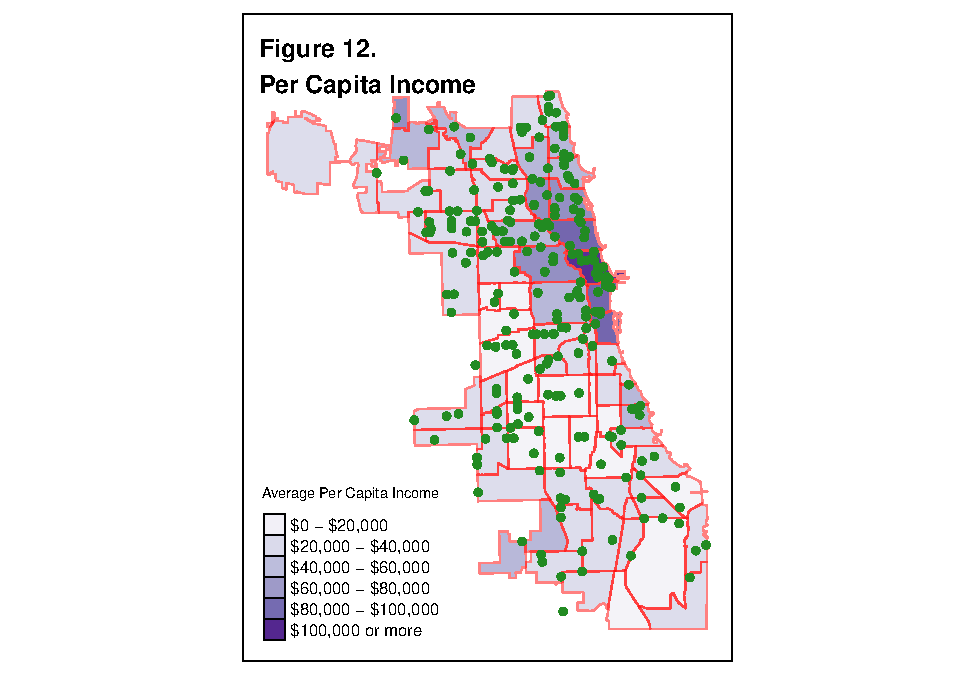
\includegraphics[width=0.5\linewidth]{Sam-Song_Coding-Sample_files/figure-latex/unnamed-chunk-12-1}
\includegraphics[width=0.5\linewidth]{Sam-Song_Coding-Sample_files/figure-latex/unnamed-chunk-12-2}

\begin{Shaded}
\begin{Highlighting}[]
\CommentTok{\# people with income less than $25,000}
\FunctionTok{tm\_shape}\NormalTok{(chicago\_sf) }\SpecialCharTok{+}
  \FunctionTok{tm\_borders}\NormalTok{(}\AttributeTok{col =} \StringTok{"red"}\NormalTok{, }\AttributeTok{alpha =}\NormalTok{ .}\DecValTok{5}\NormalTok{) }\SpecialCharTok{+}
  \FunctionTok{tm\_polygons}\NormalTok{(}\AttributeTok{col =} \StringTok{"Pct\_poverty"}\NormalTok{,}
              \AttributeTok{palette =} \StringTok{"Purples"}\NormalTok{,}
              \AttributeTok{legend.show =} \ConstantTok{FALSE}\NormalTok{) }\SpecialCharTok{+}
  \FunctionTok{tm\_shape}\NormalTok{(grocery\_store) }\SpecialCharTok{+}
    \FunctionTok{tm\_dots}\NormalTok{(}\AttributeTok{col =} \StringTok{"\#228B22"}\NormalTok{,}
          \AttributeTok{size =}\NormalTok{ .}\DecValTok{1}\NormalTok{,}
          \AttributeTok{palette =}\NormalTok{ color\_status,}
          \AttributeTok{legend.show =} \ConstantTok{FALSE}\NormalTok{) }\SpecialCharTok{+}
  \FunctionTok{tm\_layout}\NormalTok{(}\AttributeTok{title =} \StringTok{"Figure 14.}\SpecialCharTok{\textbackslash{}n}\StringTok{Percentage of Population with Income less than $25,000"}\NormalTok{,}
            \AttributeTok{inner.margins =} \FunctionTok{c}\NormalTok{(.}\DecValTok{05}\NormalTok{, .}\DecValTok{05}\NormalTok{, .}\DecValTok{12}\NormalTok{, .}\DecValTok{05}\NormalTok{),}
            \AttributeTok{title.fontface =} \StringTok{"bold"}\NormalTok{,}
            \AttributeTok{title.size =}\NormalTok{ .}\DecValTok{9}\NormalTok{) }\SpecialCharTok{+}
  \FunctionTok{tm\_add\_legend}\NormalTok{(}\AttributeTok{title =} \StringTok{"\% less than $25,000"}\NormalTok{,}
                \AttributeTok{labels =} \FunctionTok{c}\NormalTok{(}\StringTok{"0\% {-} 5\%"}\NormalTok{,}
                           \StringTok{"5\% {-} 10\%"}\NormalTok{,}
                           \StringTok{"10\% {-} 15\%"}\NormalTok{,}
                           \StringTok{"15\% {-} 20\%"}\NormalTok{,}
                           \StringTok{"20\% {-} 25\%"}\NormalTok{,}
                           \StringTok{"25\% {-} 30\%"}\NormalTok{,}
                           \StringTok{"30\% or higher"}\NormalTok{),}
                \AttributeTok{col =}\NormalTok{ RColorBrewer}\SpecialCharTok{::}\FunctionTok{brewer.pal}\NormalTok{(}\DecValTok{7}\NormalTok{, }\StringTok{"Purples"}\NormalTok{))}
\end{Highlighting}
\end{Shaded}

\begin{verbatim}
## Warning: One tm layer group has duplicated layer types, which are omitted. To
## draw multiple layers of the same type, use multiple layer groups (i.e. specify
## tm_shape prior to each of them).
\end{verbatim}

\begin{Shaded}
\begin{Highlighting}[]
\FunctionTok{ggplot}\NormalTok{(chicago\_sf) }\SpecialCharTok{+}
  \FunctionTok{geom\_point}\NormalTok{(}\FunctionTok{aes}\NormalTok{(}\AttributeTok{x =}\NormalTok{ Pct\_poverty, }\AttributeTok{y =}\NormalTok{ num\_grocery)) }\SpecialCharTok{+}
  \FunctionTok{geom\_smooth}\NormalTok{(}\FunctionTok{aes}\NormalTok{(}\AttributeTok{x =}\NormalTok{ Pct\_poverty, }\AttributeTok{y =}\NormalTok{ num\_grocery), }\AttributeTok{se =} \ConstantTok{FALSE}\NormalTok{, }\AttributeTok{method =} \StringTok{"lm"}\NormalTok{) }\SpecialCharTok{+}
  \FunctionTok{labs}\NormalTok{(}\AttributeTok{x =} \StringTok{"Poverty Rate (income less than $25,000)"}\NormalTok{,}
       \AttributeTok{y =} \StringTok{"Number of Grocery Stores"}\NormalTok{,}
       \AttributeTok{title =} \StringTok{"Figure 15. Poverty rate vs. \# of Grocery Stores"}\NormalTok{) }\SpecialCharTok{+}
  \FunctionTok{theme\_bw}\NormalTok{()}
\end{Highlighting}
\end{Shaded}

\begin{verbatim}
## `geom_smooth()` using formula = 'y ~ x'
\end{verbatim}

\includegraphics[width=0.5\linewidth]{Sam-Song_Coding-Sample_files/figure-latex/unnamed-chunk-13-1}
\includegraphics[width=0.5\linewidth]{Sam-Song_Coding-Sample_files/figure-latex/unnamed-chunk-13-2}

Figure 14 displays the average per capita income for each community
area. It seems as though the average per capita income is slightly
higher, in general, in the community areas in the north side of Chicago
than those in the south side of Chicago. But there are a few areas in
the northeast side of the city where the average per capita income is
much higher than the rest of the city, and those neighborhoods are
clusterd together. Figure 15 describes the poverty rate (people who earn
less than \$25,000 annually) of each community area. It is quite evident
that there are significantly less grocery stores in the same areas that
show high rates of poverty, and the majority of residents in these
community areas are African Americans. Looking at the scatter plot in
Figure 13 and 15, it is possible to observe the positive linear
association between the number of grocery stores and the Per Capita
Income and the negative linear association between the number of grocery
stores and the poverty rate of each community area. However, again, no
conclusions can be made before the significance testing.

\hypertarget{interactive-map}{%
\subparagraph{Interactive Map}\label{interactive-map}}

\begin{Shaded}
\begin{Highlighting}[]
\FunctionTok{tmap\_mode}\NormalTok{(}\StringTok{"view"}\NormalTok{)}
\end{Highlighting}
\end{Shaded}

\begin{verbatim}
## tmap mode set to interactive viewing
\end{verbatim}

\begin{Shaded}
\begin{Highlighting}[]
\CommentTok{\# 1. Total population}
\NormalTok{pop\_tot }\OtherTok{\textless{}{-}}\NormalTok{ chicago\_sf }\SpecialCharTok{\%\textgreater{}\%}
  \FunctionTok{select}\NormalTok{(Pop\_2020)}
\CommentTok{\# 2. White population}
\NormalTok{pct\_white }\OtherTok{\textless{}{-}}\NormalTok{ chicago\_sf }\SpecialCharTok{\%\textgreater{}\%}
  \FunctionTok{select}\NormalTok{(Pct\_white)}
\CommentTok{\# 3. Asian pouplation}
\NormalTok{pct\_asian }\OtherTok{\textless{}{-}}\NormalTok{ chicago\_sf }\SpecialCharTok{\%\textgreater{}\%}
  \FunctionTok{select}\NormalTok{(Pct\_asian)}
\CommentTok{\# 4. African American population}
\NormalTok{pct\_black }\OtherTok{\textless{}{-}}\NormalTok{ chicago\_sf }\SpecialCharTok{\%\textgreater{}\%}
  \FunctionTok{select}\NormalTok{(Pct\_black)}
\CommentTok{\# 5. Hispanic population}
\NormalTok{pct\_hispanic }\OtherTok{\textless{}{-}}\NormalTok{ chicago\_sf }\SpecialCharTok{\%\textgreater{}\%}
  \FunctionTok{select}\NormalTok{(Pct\_hispanic)}
\CommentTok{\# 6. Population of other race}
\NormalTok{pct\_other }\OtherTok{\textless{}{-}}\NormalTok{ chicago\_sf }\SpecialCharTok{\%\textgreater{}\%}
  \FunctionTok{select}\NormalTok{(Pct\_other)}
\CommentTok{\# 7. Unemployment rate}
\NormalTok{pct\_unemployed }\OtherTok{\textless{}{-}}\NormalTok{ chicago\_sf }\SpecialCharTok{\%\textgreater{}\%}
  \FunctionTok{select}\NormalTok{(Pct\_unemployed)}
\CommentTok{\# 8. Median income}
\NormalTok{median\_income }\OtherTok{\textless{}{-}}\NormalTok{ chicago\_sf }\SpecialCharTok{\%\textgreater{}\%}
  \FunctionTok{select}\NormalTok{(Med\_income)}
\CommentTok{\# 9. Per Capita income}
\NormalTok{per\_capita\_income }\OtherTok{\textless{}{-}}\NormalTok{ chicago\_sf }\SpecialCharTok{\%\textgreater{}\%}
  \FunctionTok{select}\NormalTok{(Per\_cap\_income)}
\CommentTok{\# 10. \% income less than $25,000}
\NormalTok{pct\_poverty }\OtherTok{\textless{}{-}}\NormalTok{ chicago\_sf }\SpecialCharTok{\%\textgreater{}\%}
  \FunctionTok{select}\NormalTok{(Pct\_poverty)}
\CommentTok{\# 11. \% no vehicle}
\NormalTok{pct\_no\_vehicle }\OtherTok{\textless{}{-}}\NormalTok{ chicago\_sf }\SpecialCharTok{\%\textgreater{}\%}
  \FunctionTok{select}\NormalTok{(Pct\_no\_vehicle)}


\FunctionTok{tm\_shape}\NormalTok{(chicago\_sf) }\SpecialCharTok{+}
  \FunctionTok{tm\_polygons}\NormalTok{() }\SpecialCharTok{+}
\FunctionTok{tm\_shape}\NormalTok{(pop\_tot) }\SpecialCharTok{+}
  \FunctionTok{tm\_borders}\NormalTok{(}\AttributeTok{col =} \StringTok{"red"}\NormalTok{, }\AttributeTok{alpha =}\NormalTok{ .}\DecValTok{5}\NormalTok{) }\SpecialCharTok{+}
  \FunctionTok{tm\_polygons}\NormalTok{(}\AttributeTok{col =} \StringTok{"Pop\_2020"}\NormalTok{,}
              \AttributeTok{palette =} \StringTok{"Purples"}\NormalTok{,}
              \AttributeTok{legend.show =} \ConstantTok{FALSE}\NormalTok{) }\SpecialCharTok{+}
  \FunctionTok{tm\_shape}\NormalTok{(pct\_white) }\SpecialCharTok{+}
  \FunctionTok{tm\_polygons}\NormalTok{(}\AttributeTok{col =} \StringTok{"Pct\_white"}\NormalTok{,}
              \AttributeTok{palette =} \StringTok{"Purples"}\NormalTok{,}
              \AttributeTok{legend.show =} \ConstantTok{FALSE}\NormalTok{) }\SpecialCharTok{+}
  \FunctionTok{tm\_shape}\NormalTok{(pct\_asian) }\SpecialCharTok{+}
  \FunctionTok{tm\_borders}\NormalTok{(}\AttributeTok{col =} \StringTok{"red"}\NormalTok{, }\AttributeTok{alpha =}\NormalTok{ .}\DecValTok{5}\NormalTok{) }\SpecialCharTok{+}
  \FunctionTok{tm\_polygons}\NormalTok{(}\AttributeTok{col =} \StringTok{"Pct\_asian"}\NormalTok{,}
              \AttributeTok{palette =} \StringTok{"Purples"}\NormalTok{,}
              \AttributeTok{legend.show =} \ConstantTok{FALSE}\NormalTok{) }\SpecialCharTok{+}
  \FunctionTok{tm\_shape}\NormalTok{(pct\_black) }\SpecialCharTok{+}
  \FunctionTok{tm\_borders}\NormalTok{(}\AttributeTok{col =} \StringTok{"red"}\NormalTok{, }\AttributeTok{alpha =}\NormalTok{ .}\DecValTok{5}\NormalTok{) }\SpecialCharTok{+}
  \FunctionTok{tm\_polygons}\NormalTok{(}\AttributeTok{col =} \StringTok{"Pct\_black"}\NormalTok{,}
              \AttributeTok{palette =} \StringTok{"Purples"}\NormalTok{,}
              \AttributeTok{legend.show =} \ConstantTok{FALSE}\NormalTok{) }\SpecialCharTok{+}
  \FunctionTok{tm\_shape}\NormalTok{(pct\_hispanic) }\SpecialCharTok{+}
  \FunctionTok{tm\_borders}\NormalTok{(}\AttributeTok{col =} \StringTok{"red"}\NormalTok{, }\AttributeTok{alpha =}\NormalTok{ .}\DecValTok{5}\NormalTok{) }\SpecialCharTok{+}
  \FunctionTok{tm\_polygons}\NormalTok{(}\AttributeTok{col =} \StringTok{"Pct\_hispanic"}\NormalTok{,}
              \AttributeTok{palette =} \StringTok{"Purples"}\NormalTok{,}
              \AttributeTok{legend.show =} \ConstantTok{FALSE}\NormalTok{) }\SpecialCharTok{+}
  \FunctionTok{tm\_shape}\NormalTok{(pct\_other) }\SpecialCharTok{+}
  \FunctionTok{tm\_borders}\NormalTok{(}\AttributeTok{col =} \StringTok{"red"}\NormalTok{, }\AttributeTok{alpha =}\NormalTok{ .}\DecValTok{5}\NormalTok{) }\SpecialCharTok{+}
  \FunctionTok{tm\_polygons}\NormalTok{(}\AttributeTok{col =} \StringTok{"Pct\_other"}\NormalTok{,}
              \AttributeTok{palette =} \StringTok{"Purples"}\NormalTok{,}
              \AttributeTok{legend.show =} \ConstantTok{FALSE}\NormalTok{) }\SpecialCharTok{+}
  \FunctionTok{tm\_shape}\NormalTok{(pct\_unemployed) }\SpecialCharTok{+}
  \FunctionTok{tm\_borders}\NormalTok{(}\AttributeTok{col =} \StringTok{"red"}\NormalTok{, }\AttributeTok{alpha =}\NormalTok{ .}\DecValTok{5}\NormalTok{) }\SpecialCharTok{+}
  \FunctionTok{tm\_polygons}\NormalTok{(}\AttributeTok{col =} \StringTok{"Pct\_unemployed"}\NormalTok{,}
              \AttributeTok{palette =} \StringTok{"Purples"}\NormalTok{,}
              \AttributeTok{legend.show =} \ConstantTok{FALSE}\NormalTok{) }\SpecialCharTok{+}
    \FunctionTok{tm\_shape}\NormalTok{(median\_income) }\SpecialCharTok{+}
  \FunctionTok{tm\_borders}\NormalTok{(}\AttributeTok{col =} \StringTok{"red"}\NormalTok{, }\AttributeTok{alpha =}\NormalTok{ .}\DecValTok{5}\NormalTok{) }\SpecialCharTok{+}
  \FunctionTok{tm\_polygons}\NormalTok{(}\AttributeTok{col =} \StringTok{"Med\_income"}\NormalTok{,}
              \AttributeTok{palette =} \StringTok{"Purples"}\NormalTok{,}
              \AttributeTok{legend.show =} \ConstantTok{FALSE}\NormalTok{) }\SpecialCharTok{+}
  \FunctionTok{tm\_shape}\NormalTok{(per\_capita\_income) }\SpecialCharTok{+}
  \FunctionTok{tm\_borders}\NormalTok{(}\AttributeTok{col =} \StringTok{"red"}\NormalTok{, }\AttributeTok{alpha =}\NormalTok{ .}\DecValTok{5}\NormalTok{) }\SpecialCharTok{+}
  \FunctionTok{tm\_polygons}\NormalTok{(}\AttributeTok{col =} \StringTok{"Per\_cap\_income"}\NormalTok{,}
              \AttributeTok{palette =} \StringTok{"Purples"}\NormalTok{,}
              \AttributeTok{legend.show =} \ConstantTok{FALSE}\NormalTok{) }\SpecialCharTok{+}
  \FunctionTok{tm\_shape}\NormalTok{(pct\_poverty) }\SpecialCharTok{+}
  \FunctionTok{tm\_borders}\NormalTok{(}\AttributeTok{col =} \StringTok{"red"}\NormalTok{, }\AttributeTok{alpha =}\NormalTok{ .}\DecValTok{5}\NormalTok{) }\SpecialCharTok{+}
  \FunctionTok{tm\_polygons}\NormalTok{(}\AttributeTok{col =} \StringTok{"Pct\_poverty"}\NormalTok{,}
              \AttributeTok{palette =} \StringTok{"Purples"}\NormalTok{,}
              \AttributeTok{legend.show =} \ConstantTok{FALSE}\NormalTok{) }\SpecialCharTok{+}
    \FunctionTok{tm\_shape}\NormalTok{(pct\_no\_vehicle) }\SpecialCharTok{+}
  \FunctionTok{tm\_borders}\NormalTok{(}\AttributeTok{col =} \StringTok{"red"}\NormalTok{, }\AttributeTok{alpha =}\NormalTok{ .}\DecValTok{5}\NormalTok{) }\SpecialCharTok{+}
  \FunctionTok{tm\_polygons}\NormalTok{(}\AttributeTok{col =} \StringTok{"Pct\_no\_vehicle"}\NormalTok{,}
              \AttributeTok{palette =} \StringTok{"Purples"}\NormalTok{,}
              \AttributeTok{legend.show =} \ConstantTok{FALSE}\NormalTok{) }\SpecialCharTok{+}
  \FunctionTok{tm\_shape}\NormalTok{(grocery\_store) }\SpecialCharTok{+}
  \FunctionTok{tm\_dots}\NormalTok{(}\AttributeTok{col =} \StringTok{"\#228B22"}\NormalTok{,}
          \AttributeTok{size =}\NormalTok{ .}\DecValTok{03}\NormalTok{,}
          \AttributeTok{legend.show =} \ConstantTok{FALSE}\NormalTok{)}
\end{Highlighting}
\end{Shaded}

\begin{verbatim}
## Warning: One tm layer group has duplicated layer types, which are omitted. To
## draw multiple layers of the same type, use multiple layer groups (i.e. specify
## tm_shape prior to each of them).

## Warning: One tm layer group has duplicated layer types, which are omitted. To
## draw multiple layers of the same type, use multiple layer groups (i.e. specify
## tm_shape prior to each of them).

## Warning: One tm layer group has duplicated layer types, which are omitted. To
## draw multiple layers of the same type, use multiple layer groups (i.e. specify
## tm_shape prior to each of them).

## Warning: One tm layer group has duplicated layer types, which are omitted. To
## draw multiple layers of the same type, use multiple layer groups (i.e. specify
## tm_shape prior to each of them).

## Warning: One tm layer group has duplicated layer types, which are omitted. To
## draw multiple layers of the same type, use multiple layer groups (i.e. specify
## tm_shape prior to each of them).

## Warning: One tm layer group has duplicated layer types, which are omitted. To
## draw multiple layers of the same type, use multiple layer groups (i.e. specify
## tm_shape prior to each of them).

## Warning: One tm layer group has duplicated layer types, which are omitted. To
## draw multiple layers of the same type, use multiple layer groups (i.e. specify
## tm_shape prior to each of them).

## Warning: One tm layer group has duplicated layer types, which are omitted. To
## draw multiple layers of the same type, use multiple layer groups (i.e. specify
## tm_shape prior to each of them).

## Warning: One tm layer group has duplicated layer types, which are omitted. To
## draw multiple layers of the same type, use multiple layer groups (i.e. specify
## tm_shape prior to each of them).

## Warning: One tm layer group has duplicated layer types, which are omitted. To
## draw multiple layers of the same type, use multiple layer groups (i.e. specify
## tm_shape prior to each of them).
\end{verbatim}

This is an interactive map where the user can change the input of their
interests and look into the distribution of demographic factors
throughout the city of Chicago, overlaid with the grocery store
locations, which could hint at the spatial association between the
grocery store locations and other demographic factors that I did not
include in this analysis. \textbf{Click one variable of interest at a
time other than \texttt{grocery\ store}.}

\hypertarget{regression}{%
\subsubsection{Regression}\label{regression}}

To test the significance of the independent variables in their
relationship with the number of grocery stores in each community area, I
started by fitting regular linear regression models first.

\begin{Shaded}
\begin{Highlighting}[]
\NormalTok{chicago\_sf }\OtherTok{\textless{}{-}}\NormalTok{ chicago\_sf }\SpecialCharTok{\%\textgreater{}\%}
  \FunctionTok{mutate}\NormalTok{(}\AttributeTok{income1000 =}\NormalTok{ Per\_cap\_income }\SpecialCharTok{/} \DecValTok{1000}\NormalTok{)}
\end{Highlighting}
\end{Shaded}

\begin{Shaded}
\begin{Highlighting}[]
\NormalTok{pct\_white\_lm }\OtherTok{\textless{}{-}} \FunctionTok{lm}\NormalTok{(num\_grocery }\SpecialCharTok{\textasciitilde{}}\NormalTok{ Pct\_white, }\AttributeTok{data =}\NormalTok{ chicago\_sf)}
\FunctionTok{summary}\NormalTok{(pct\_white\_lm)}
\end{Highlighting}
\end{Shaded}

\begin{verbatim}
## 
## Call:
## lm(formula = num_grocery ~ Pct_white, data = chicago_sf)
## 
## Residuals:
##     Min      1Q  Median      3Q     Max 
## -4.1192 -1.9137 -0.4893  1.2508 10.6488 
## 
## Coefficients:
##             Estimate Std. Error t value Pr(>|t|)    
## (Intercept)  2.25352    0.48603   4.637 1.47e-05 ***
## Pct_white    0.03358    0.01279   2.626   0.0105 *  
## ---
## Signif. codes:  0 '***' 0.001 '**' 0.01 '*' 0.05 '.' 0.1 ' ' 1
## 
## Residual standard error: 2.927 on 75 degrees of freedom
## Multiple R-squared:  0.08419,    Adjusted R-squared:  0.07198 
## F-statistic: 6.895 on 1 and 75 DF,  p-value: 0.01047
\end{verbatim}

\begin{Shaded}
\begin{Highlighting}[]
\NormalTok{pct\_black\_lm }\OtherTok{\textless{}{-}} \FunctionTok{lm}\NormalTok{(num\_grocery }\SpecialCharTok{\textasciitilde{}}\NormalTok{ Pct\_black, }\AttributeTok{data =}\NormalTok{ chicago\_sf)}
\FunctionTok{summary}\NormalTok{(pct\_black\_lm)}
\end{Highlighting}
\end{Shaded}

\begin{verbatim}
## 
## Call:
## lm(formula = num_grocery ~ Pct_black, data = chicago_sf)
## 
## Residuals:
##     Min      1Q  Median      3Q     Max 
## -4.1902 -1.9168 -0.5258  0.8746 10.9073 
## 
## Coefficients:
##              Estimate Std. Error t value Pr(>|t|)    
## (Intercept)  4.286280   0.447768   9.573 1.22e-14 ***
## Pct_black   -0.030881   0.008688  -3.555 0.000659 ***
## ---
## Signif. codes:  0 '***' 0.001 '**' 0.01 '*' 0.05 '.' 0.1 ' ' 1
## 
## Residual standard error: 2.829 on 75 degrees of freedom
## Multiple R-squared:  0.1442, Adjusted R-squared:  0.1328 
## F-statistic: 12.63 on 1 and 75 DF,  p-value: 0.0006594
\end{verbatim}

\begin{Shaded}
\begin{Highlighting}[]
\NormalTok{per\_cap\_income\_lm }\OtherTok{\textless{}{-}} \FunctionTok{lm}\NormalTok{(num\_grocery }\SpecialCharTok{\textasciitilde{}}\NormalTok{ income1000, }\AttributeTok{data =}\NormalTok{ chicago\_sf)}
\FunctionTok{summary}\NormalTok{(per\_cap\_income\_lm)}
\end{Highlighting}
\end{Shaded}

\begin{verbatim}
## 
## Call:
## lm(formula = num_grocery ~ income1000, data = chicago_sf)
## 
## Residuals:
##    Min     1Q Median     3Q    Max 
## -4.786 -1.850 -0.363  1.121 10.658 
## 
## Coefficients:
##             Estimate Std. Error t value Pr(>|t|)    
## (Intercept)  0.91187    0.62577   1.457    0.149    
## income1000   0.06616    0.01578   4.192 7.47e-05 ***
## ---
## Signif. codes:  0 '***' 0.001 '**' 0.01 '*' 0.05 '.' 0.1 ' ' 1
## 
## Residual standard error: 2.753 on 75 degrees of freedom
## Multiple R-squared:  0.1898, Adjusted R-squared:  0.179 
## F-statistic: 17.58 on 1 and 75 DF,  p-value: 7.474e-05
\end{verbatim}

\begin{Shaded}
\begin{Highlighting}[]
\NormalTok{pct\_poverty\_lm }\OtherTok{\textless{}{-}} \FunctionTok{lm}\NormalTok{(num\_grocery }\SpecialCharTok{\textasciitilde{}}\NormalTok{ Pct\_poverty, }\AttributeTok{data =}\NormalTok{ chicago\_sf)}
\FunctionTok{summary}\NormalTok{(pct\_poverty\_lm)}
\end{Highlighting}
\end{Shaded}

\begin{verbatim}
## 
## Call:
## lm(formula = num_grocery ~ Pct_poverty, data = chicago_sf)
## 
## Residuals:
##     Min      1Q  Median      3Q     Max 
## -4.3695 -1.9306 -0.6913  1.0628 11.3665 
## 
## Coefficients:
##             Estimate Std. Error t value Pr(>|t|)    
## (Intercept)   4.8597     0.6982   6.960  1.1e-09 ***
## Pct_poverty  -0.1650     0.0604  -2.732  0.00784 ** 
## ---
## Signif. codes:  0 '***' 0.001 '**' 0.01 '*' 0.05 '.' 0.1 ' ' 1
## 
## Residual standard error: 2.917 on 75 degrees of freedom
## Multiple R-squared:  0.09053,    Adjusted R-squared:  0.07841 
## F-statistic: 7.466 on 1 and 75 DF,  p-value: 0.007837
\end{verbatim}

To briefly touch on the results of a series of linear regressions, all
four independent variables of my interests (\% white, \%
African-american, Per capita income, and Poverty rate) are significant
predictors of the number of grocery stores in each community area.
Interpretations of linear regression specific to each independent
variable are as follows:

\begin{enumerate}
\def\labelenumi{\arabic{enumi}.}
\tightlist
\item
  For every 1\% increase in the percentage of White residents, the mean
  number of grocery stores increases by about 0.03 (p-value = 0.021).\\
\item
  For every 1\% increase in the percentage of African-american
  residents, the mean number of grocery stores decreases by about 0.03
  (p-value = 0.002).\\
\item
  For every \$1,000 increase in the per capita income, the mean number
  of grocery stores increases by about 1.07 (p-value = 0.0002).\\
\item
  For every 1\% increase in the percentage of residents earning less
  than \$25,000, the mean number of grocery stores decreases by about
  0.16 (p-value = 0.014).
\end{enumerate}

\hypertarget{simultaneous-autoregressive-model}{%
\subsubsection{Simultaneous Autoregressive
Model}\label{simultaneous-autoregressive-model}}

While the job seems to be done with the significant results above, we
should not forget that we are dealing with spatial data. Therefore, it
is necessary to test the existence of spatial autocorrelation. As
mentioned before, if the spatial autocorrelation exists and is high, it
needs to be accounted by using simultaneous autoregressive model.
Otherwise, the assumption of independence, one of the conditions that
have to be met to trust the results of linear regression, is violated.
Below are the results from the simultaneous autoregressive models.

\begin{Shaded}
\begin{Highlighting}[]
\NormalTok{sarlm\_white }\OtherTok{\textless{}{-}} \FunctionTok{lagsarlm}\NormalTok{(num\_grocery }\SpecialCharTok{\textasciitilde{}}\NormalTok{ Pct\_white, }\AttributeTok{data =}\NormalTok{ chicago\_sf, }\AttributeTok{listw =}\NormalTok{ chicago\_nbw)}
\FunctionTok{summary}\NormalTok{(sarlm\_white)}
\end{Highlighting}
\end{Shaded}

\begin{verbatim}
## 
## Call:lagsarlm(formula = num_grocery ~ Pct_white, data = chicago_sf, 
##     listw = chicago_nbw)
## 
## Residuals:
##      Min       1Q   Median       3Q      Max 
## -5.18597 -1.79870 -0.40542  1.04918 10.04833 
## 
## Type: lag 
## Coefficients: (asymptotic standard errors) 
##             Estimate Std. Error z value Pr(>|z|)
## (Intercept) 1.159508   0.541014  2.1432   0.0321
## Pct_white   0.018964   0.011918  1.5912   0.1116
## 
## Rho: 0.45555, LR test value: 10.118, p-value: 0.0014684
## Asymptotic standard error: 0.13075
##     z-value: 3.4842, p-value: 0.00049358
## Wald statistic: 12.14, p-value: 0.00049358
## 
## Log likelihood: -185.8734 for lag model
## ML residual variance (sigma squared): 6.973, (sigma: 2.6406)
## Number of observations: 77 
## Number of parameters estimated: 4 
## AIC: NA (not available for weighted model), (AIC for lm: 387.86)
## LM test for residual autocorrelation
## test value: 2.8694, p-value: 0.090278
\end{verbatim}

\begin{Shaded}
\begin{Highlighting}[]
\NormalTok{sarlm\_black }\OtherTok{\textless{}{-}} \FunctionTok{lagsarlm}\NormalTok{(num\_grocery }\SpecialCharTok{\textasciitilde{}}\NormalTok{ Pct\_black, }\AttributeTok{data =}\NormalTok{ chicago\_sf, }\AttributeTok{listw =}\NormalTok{ chicago\_nbw)}
\FunctionTok{summary}\NormalTok{(sarlm\_black)}
\end{Highlighting}
\end{Shaded}

\begin{verbatim}
## 
## Call:lagsarlm(formula = num_grocery ~ Pct_black, data = chicago_sf, 
##     listw = chicago_nbw)
## 
## Residuals:
##      Min       1Q   Median       3Q      Max 
## -5.49268 -1.67312 -0.55633  1.04410  9.60536 
## 
## Type: lag 
## Coefficients: (asymptotic standard errors) 
##               Estimate Std. Error z value  Pr(>|z|)
## (Intercept)  2.5664129  0.6668712  3.8484 0.0001189
## Pct_black   -0.0202729  0.0085562 -2.3694 0.0178174
## 
## Rho: 0.40763, LR test value: 7.8876, p-value: 0.0049775
## Asymptotic standard error: 0.13498
##     z-value: 3.0201, p-value: 0.0025273
## Wald statistic: 9.1207, p-value: 0.0025273
## 
## Log likelihood: -184.3804 for lag model
## ML residual variance (sigma squared): 6.7779, (sigma: 2.6034)
## Number of observations: 77 
## Number of parameters estimated: 4 
## AIC: NA (not available for weighted model), (AIC for lm: 382.65)
## LM test for residual autocorrelation
## test value: 1.2581, p-value: 0.26201
\end{verbatim}

\begin{Shaded}
\begin{Highlighting}[]
\NormalTok{sarlm\_per\_cap\_income }\OtherTok{\textless{}{-}} \FunctionTok{lagsarlm}\NormalTok{(num\_grocery }\SpecialCharTok{\textasciitilde{}}\NormalTok{ income1000, }\AttributeTok{data =}\NormalTok{ chicago\_sf, }\AttributeTok{listw =}\NormalTok{ chicago\_nbw)}
\FunctionTok{summary}\NormalTok{(sarlm\_per\_cap\_income)}
\end{Highlighting}
\end{Shaded}

\begin{verbatim}
## 
## Call:lagsarlm(formula = num_grocery ~ income1000, data = chicago_sf, 
##     listw = chicago_nbw)
## 
## Residuals:
##      Min       1Q   Median       3Q      Max 
## -4.43027 -1.77474 -0.39477  0.92216 10.39496 
## 
## Type: lag 
## Coefficients: (asymptotic standard errors) 
##             Estimate Std. Error z value Pr(>|z|)
## (Intercept) 0.369195   0.630457  0.5856 0.558145
## income1000  0.046726   0.015754  2.9660 0.003017
## 
## Rho: 0.36781, LR test value: 6.2974, p-value: 0.012091
## Asymptotic standard error: 0.1391
##     z-value: 2.6442, p-value: 0.0081876
## Wald statistic: 6.992, p-value: 0.0081876
## 
## Log likelihood: -183.0641 for lag model
## ML residual variance (sigma squared): 6.5994, (sigma: 2.5689)
## Number of observations: 77 
## Number of parameters estimated: 4 
## AIC: NA (not available for weighted model), (AIC for lm: 378.43)
## LM test for residual autocorrelation
## test value: 5.5531, p-value: 0.018448
\end{verbatim}

\begin{Shaded}
\begin{Highlighting}[]
\NormalTok{sarlm\_poverty }\OtherTok{\textless{}{-}} \FunctionTok{lagsarlm}\NormalTok{(num\_grocery }\SpecialCharTok{\textasciitilde{}}\NormalTok{ Pct\_poverty, }\AttributeTok{data =}\NormalTok{ chicago\_sf, }\AttributeTok{listw =}\NormalTok{ chicago\_nbw)}
\FunctionTok{summary}\NormalTok{(sarlm\_poverty)}
\end{Highlighting}
\end{Shaded}

\begin{verbatim}
## 
## Call:lagsarlm(formula = num_grocery ~ Pct_poverty, data = chicago_sf, 
##     listw = chicago_nbw)
## 
## Residuals:
##      Min       1Q   Median       3Q      Max 
## -5.21852 -1.59665 -0.63306  1.11119  9.74928 
## 
## Type: lag 
## Coefficients: (asymptotic standard errors) 
##              Estimate Std. Error z value  Pr(>|z|)
## (Intercept)  2.707736   0.821263  3.2970 0.0009771
## Pct_poverty -0.099946   0.055843 -1.7898 0.0734934
## 
## Rho: 0.45318, LR test value: 10.202, p-value: 0.0014027
## Asymptotic standard error: 0.13026
##     z-value: 3.479, p-value: 0.0005033
## Wald statistic: 12.103, p-value: 0.0005033
## 
## Log likelihood: -185.5636 for lag model
## ML residual variance (sigma squared): 6.9209, (sigma: 2.6308)
## Number of observations: 77 
## Number of parameters estimated: 4 
## AIC: NA (not available for weighted model), (AIC for lm: 387.33)
## LM test for residual autocorrelation
## test value: 2.9642, p-value: 0.085129
\end{verbatim}

All four of models return \(\rho\) values between 0.33 and 0.42 with
their respective p-values less than 0.05. Such moderately positive
\(\rho\) values tell us that there does exists the difference, though
not by much, in the results between SAR model and linear regression
model. Therefore, it might be a good idea that we take into account of
spatial autocorrelation when interpreting the regression results and
making conclusions.

Interpretations of SAR models specific to each independent variable are
as follows:

\begin{enumerate}
\def\labelenumi{\arabic{enumi}.}
\item
  After accounting for spatial autocorrelation between neighboring
  community areas, the p-value for the percentage of white residents is
  greater than 0.05. Therefore, we fail to reject the null hypothesis
  and conclude that this is not a statistically significant predictor
  for the number of grocery stores in each community area of Chicago.
  (p-value = 0.135)\\
\item
  After accounting for spatial autocorrelation between neighboring
  community areas, for every 1\% increase in the percentage of
  African-american residents, the mean number of grocery stores
  decreases by about 0.02 (p-value = 0.03).\\
\end{enumerate}

3.After accounting for spatial autocorrelation between neighboring
community areas, for every \$1,000 increase in the per capita income,
the mean number of grocery stores increases by about 0.05 (p-value =
0.004).\\

\begin{enumerate}
\def\labelenumi{\arabic{enumi}.}
\setcounter{enumi}{3}
\tightlist
\item
  After accounting for spatial autocorrelation between neighboring
  community areas, the p-value for the poverty rate is greater than
  0.05. Therefore, we fail to reject the null hypothesis and conclude
  that this is not a statistically significant predictor for the number
  of grocery stores in each community area of Chicago. (p-value =
  0.09).\\
\end{enumerate}

To sum up, the results have changed after the use of SAR model, which
accounted for the spatial correlations. Two of the variables (percentage
of white residents and percentage of residents earning less than
\$25,000) that were significant in the linear regression are no longer
significant under SAR model. However, the other two variables
(percentage of African-american residents and Per capita income) remain
significant even after considering the spatial autocorrelation.
Therefore, percentage of African-american residents and the per capita
income of each of the community area of Chicago can be statistically
significant predictors of the number of grocery stores in the area.

\hypertarget{about-ecological-fallacy}{%
\subsubsection{About Ecological
Fallacy}\label{about-ecological-fallacy}}

An Ecological Fallacy is a formal fallacy in the interpretation of
statistical data that occurs when if the observed relationships at
aggregate (group) levels are falsely attributed to individual levels.
This should be avoided because it can lead to erroneous conclusions and
false assumptions about relationships especially in social phenomena. An
Ecological Fallacy can also be used to justify the false belief or
assumption.

In the case of this analysis, all of the demographic data and the number
of grocery stores are aggregated at the community area level. Therefore,
all conclusions regarding spatial autocorrelation and the significance
of demographic factors in relation to the number of grocery stores
should not be applied to smaller neighborhoods, household, or individual
levels. It is likely that the results could change (possibly
drastically) if the same analysis would be done with data gathered at
different aggregate levels.

\end{document}
